\documentclass[a4paper,12pt]{report}
\usepackage{graphicx}
\usepackage{hyperref}
\usepackage[utf8]{inputenc}
\usepackage{url}
\usepackage{pdfpages}
\usepackage[italian]{babel}
\usepackage[italian]{cleveref}
\usepackage{float}

\title{Elaborato per il corso Basi di Dati\\ \small Progetto di una base di dati per la gestione di un sito di e-Commerce}

\author{
    Studente: Emma Leonardi\\
    Email: \url{emma.leonardi2@studio.unibo.it}\\
    Matricola: 0000971438\\
    A.A. 2021/2022
    }
\date{}
\begin{document}

\maketitle
\tableofcontents

\chapter{Analisi}
\section{Analisi dei requisiti}
Si ha intenzione di creare un database per gestire un sito di e-Commerce.
Il database dovrà memorizzare informazioni sui prodotti in vendita, gestire l'interazione con il cliente che compra i prodotti. 
Inoltre dovrà gestire anche i corrieri che effettuano le consegne delle spese e sapere in quale fabbrica viene prodotto quale prodotto.
\section{Intervista}
Si vuole tenere traccia degli acquisti dei clienti. I dati dei clienti memorizzati sono nome, cognome, codice fiscale, data di nascita, 
email e numero di telefono, coordinate bancarie e indirizzo di residenza.
Il cliente acquista un'insieme di prodotti con un costo che è la somma dei costi singoli. 
I prodotti possono cambiare prezzo nel tempo e bisogna tenere memorizzato lo storico. 
Dei prodotti si salva il materiale, la descrizione, la taglia se abbigliamento o la scadenza se prodotto alimentare. 
I prodotti vengono creati in fabbriche, gestite da più produttori in periodi diversi. Una fabbrica viene gestita da un solo amministratore alla volta e può produrre diversi prodotti. 
Del produttore si salva la partita IVA e della fabbrica l'indirizzo. Un prodotto viene fabbricato in una sola fabbrica.
La spesa viene consegnata da un corriere e si salva la data. Un autista guida un mezzo per fare le spedizioni, di cui si memorizzano il tipo di veicolo, la marca, il paese di immatricolazione e la targa.
Del corriere vengono memorizzate la nazionalità della patente, il codice e i turni di guida. La consegna può essere standard o premium, e cambia il prezzo.
La consegna ha collegato un indirizzo, che può essere diverso dall'indirizzo di residenza del cliente. Più autisti non possono guidare lo stesso furgone in contemporanea, la consegna è effettuata da un unico corriere 
e si riferisce ad una sola spesa. Una spesa è riferita a un solo acquirente, ma un cliente può effettuare più spese. 
Si memorizzano nome, cognome, codice fiscale e data di nascita per i clienti, produttori e corrieri.

\section{Rilevamento delle ambiguità e correzioni proposte}
\begin{center}
    \begin{tabular}{ | c | c | c |} 
    \hline
    Termine&Descrizione&Sinonimi \\
    \hline
    Cliente&Una persona che usa il sistema per acquistare prodotti&Acquirente \\
	\hline
	Spesa&L'insieme dei prodotti acquistati insieme da un cliente&...\\
	\hline
	Prodotto&Un articolo in vendita&Oggetto\\
	\hline
	Produttore&Una persona che gestisce una fabbrica&Amministratore\\
	\hline
	Corriere&Una persona che guida un mezzo e fa consegne&Autista\\
	\hline
	Mezzo&Un mezzo di trasporto per fare le consegne&Veicolo\\
	\hline
	Consegna&Una spesa in arrivo o arrivata al cliente&Spedizione\\
	\hline
    \end{tabular}
\end{center}
\section{Definizione delle specifiche in linguaggio naturale ed estrazione dei concetti principali}
Usando la tabella sopra, rimuovo l'ambiguità dal testo dell'intervista.\\

Si vuole tenere traccia degli acquisti dei clienti. I dati dei clienti memorizzati sono nome, cognome, codice fiscale, data di nascita, 
email e numero di telefono, coordinate bancarie e indirizzo di residenza.
Il cliente acquista una spesa con un costo che è la somma dei costi dei prodotti presenti nella spesa. 
I prodotti possono cambiare prezzo nel tempo e bisogna tenere memorizzato lo storico. 
Dei prodotti si salva il materiale, la descrizione, la taglia se abbigliamento o la scadenza se prodotto alimentare. 
I prodotti vengono creati in fabbriche, gestite da più produttori in periodi diversi. Una fabbrica viene gestita da un solo produttore alla volta e può produrre diversi prodotti. 
Del produttore si salva la partita IVA e della fabbrica l'indirizzo. Un prodotto viene fabbricato in una sola fabbrica.
La spesa viene consegnata da un corriere e si salva la data. Un corriere guida un mezzo, di cui si memorizzano il tipo di veicolo, la marca, il paese di immatricolazione e la targa.
Del corriere vengono memorizzate la nazionalità della patente, il codice e i turni di guida. La consegna può essere standard o premium, cambia il prezzo della consegna.
La consegna ha collegato un indirizzo, che può essere diverso dall'indirizzo di residenza del cliente. Più corrieri non possono guidare lo stesso mezzo in contemporanea, la consegna è effettuata da un unico corriere 
e si riferisce ad una sola spesa. Una spesa è riferita a un solo cliente, ma un cliente può effettuare più spese. 
Si memorizzano nome, cognome, codice fiscale e data di nascita per i clienti, produttori e corrieri.

\chapter{Progettazione Concettuale}
\section{Clienti}
\subsection{Schema scheletro}
Dopo aver esaminato il dominio del problema per la parte dei clienti, viene proposto il seguente schema scheletro.
\begin{figure}[H]
	\centering{}
	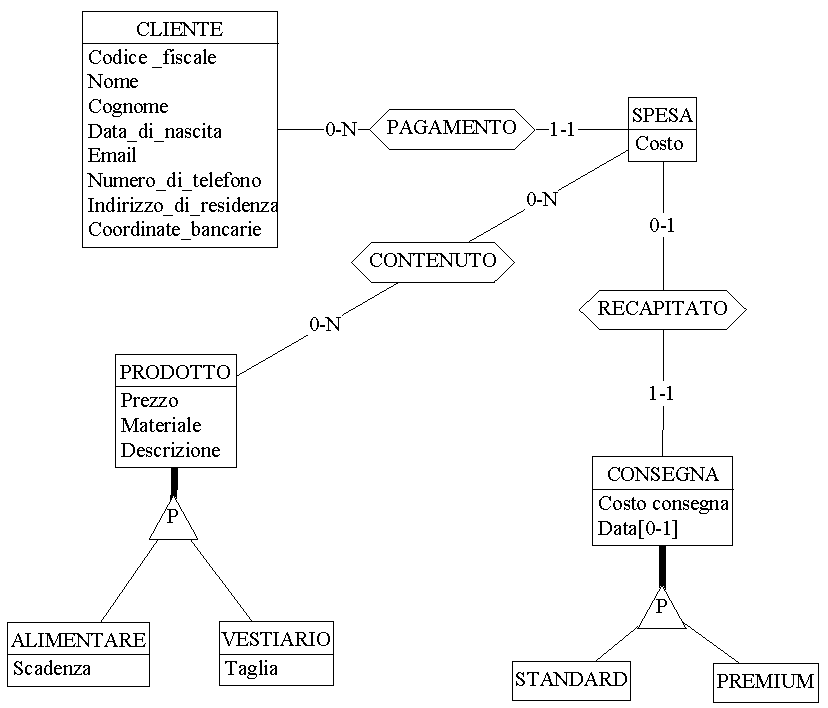
\includegraphics[width=\textwidth]{img/SchemaConcettuale-Clienti1.pdf}
	\caption{Schema scheletro per i Clienti}
\end{figure}
\subsection{Raffinamenti proposti}
L'entità Cliente è una estensione di un'entità generica Persona, che si decide di aggiungere allo schema. 
L'entità Prodotto non permette di mantenere uno storico dei diversi prezzi e delle diverse "versioni" dello stesso prodotto, come la taglia o la scadenza. 
Per questo si decide di creare un'entità Prodotto in Vendita che è il prodotto venduto al cliente, collegato a Prodotto via Commercializzato e si aggiungono al Prodotto in Vendita il prezzo e il periodo di validità del prezzo. 
Come identificatori per l'entità cliente si usa un codice univoco (per evitare l'omocodia del codice fiscale), per Spesa e Prodotto e Consegna si usa un codice univoco. Prodotto In Vendita usa come identificatore l'identificatore di Prodotto e la data di inizio di vendita.
\subsection{Schema concettuale parziale}
\begin{figure}[H]
	\centering{}
	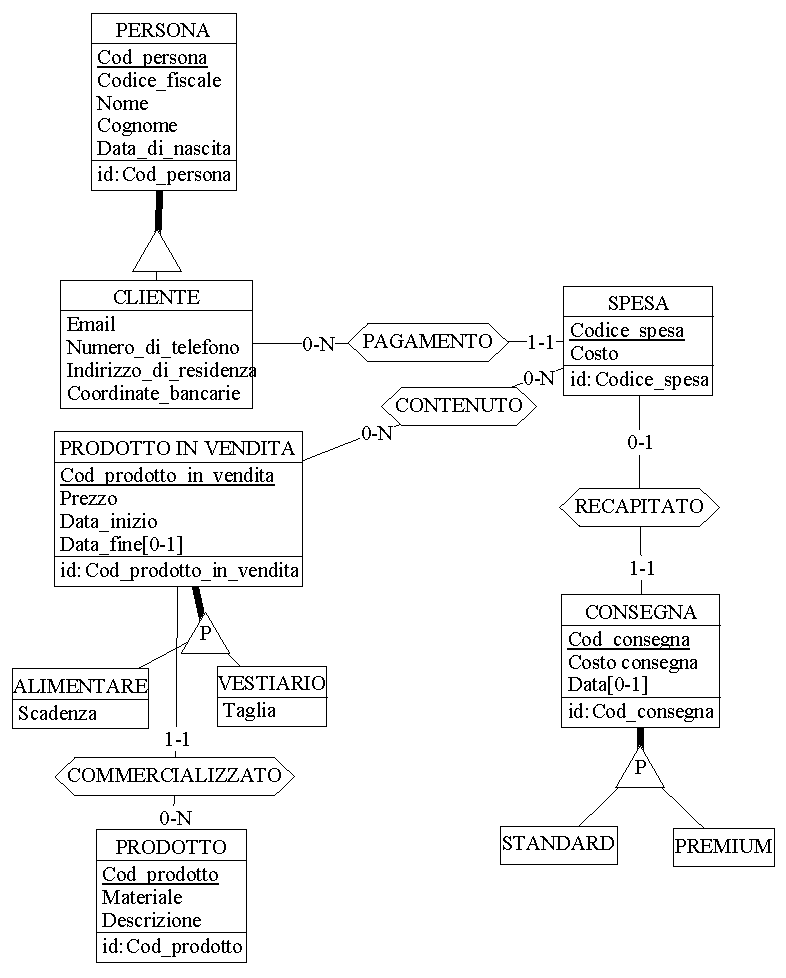
\includegraphics[width=\textwidth]{img/SchemaConcettuale-Clienti2.pdf}
	\caption{Schema scheletro per i Clienti, dopo le modifiche apportate}
\end{figure}
\section{Corrieri}
\subsection{Schema scheletro}
Dopo aver esaminato il dominio del problema per la parte dei corrieri, viene proposto il seguente schema scheletro.
\begin{figure}[H]
	\centering{}
	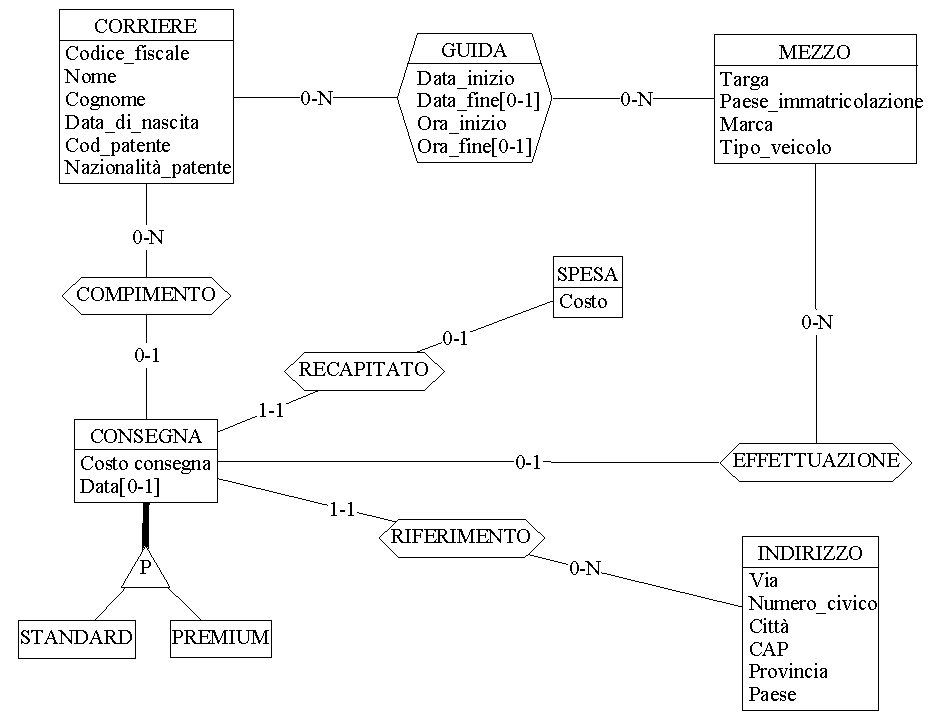
\includegraphics[width=\textwidth]{img/SchemaConcettuale-Corrieri1.pdf}
	\caption{Schema scheletro per i Corrieri}
\end{figure}
\subsection{Raffinamenti proposti}
L'entità Corriere è una estensione di un'entità generica Persona, che si decide di aggiungere allo schema. 
La relazione Guida non è corretta rappresentata come relazione perchè questo impedisce ad un corriere di guidare lo stesso mezzo più volte. 
Guida diventa una entità quindi, in relazione 1-1 con Corriere attraverso Conducente e attraverso Utilizzo per Mezzo, mentre le cardinalità dai lati delle entità rimangono 0-N. 
Come identificatori per Corriere si può usare il codice di persona oppure il codice della patente. 
Per Mezzo come identificatore uso la Targa, per Consegna,Spesa e Indirizzo un codice univoco. 
Gli identificatori di guida sono due i possibili, o l'identificatore di Corriere unito alla data ed ora oppure l'identificatore di Mezzo unito alla data ed ora. 
Un vincolo inespresso è il fatto che più guide dello stesso corriere possono avvenire contemporaneamente. 
\subsection{Schema concettuale parziale}
\begin{figure}[H]
	\centering{}
	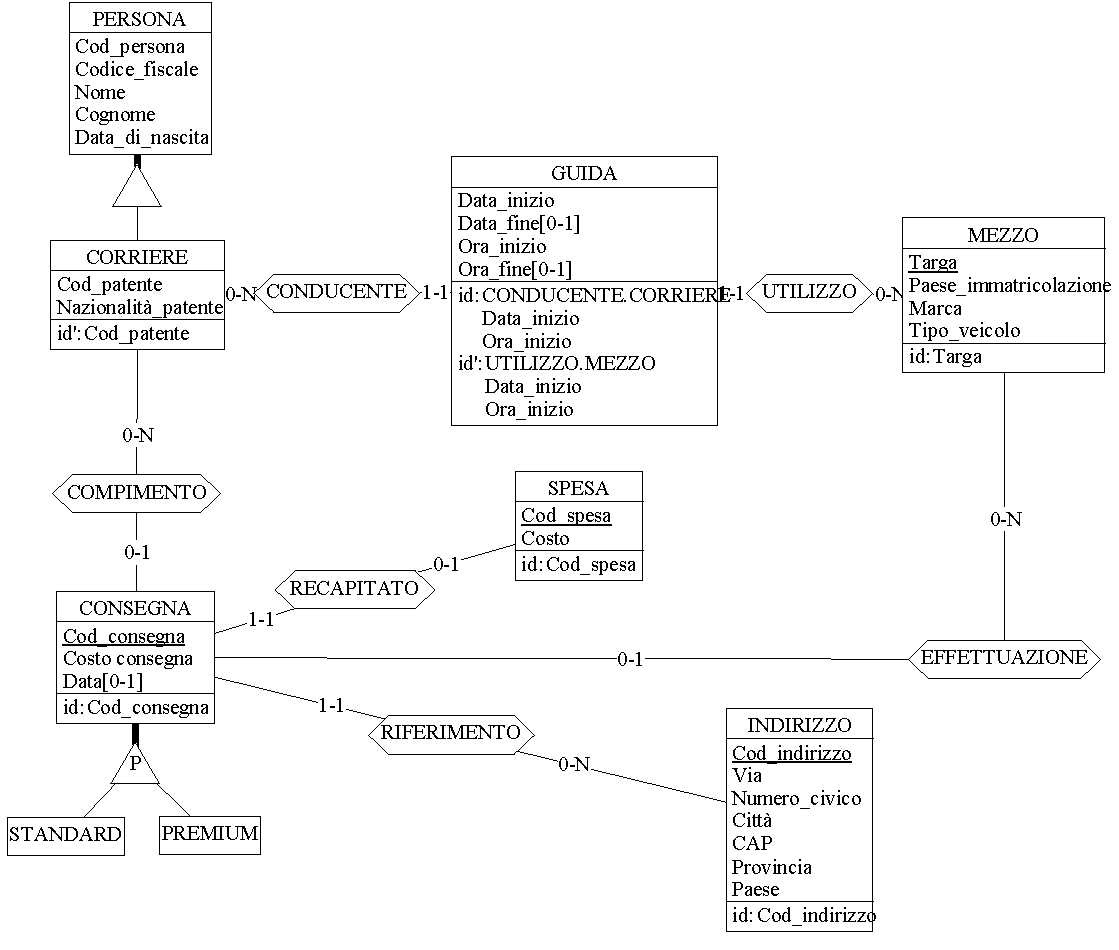
\includegraphics[width=\textwidth]{img/SchemaConcettuale-Corrieri2.pdf}
	\caption{Schema scheletro per i Corrieri, dopo le modifiche apportate}
\end{figure}
\section{Produttore}
\subsection{Schema scheletro}
Dopo aver esaminato il dominio del problema per la parte dei produttori, viene proposto il seguente schema scheletro.
\begin{figure}[H]
	\centering{}
	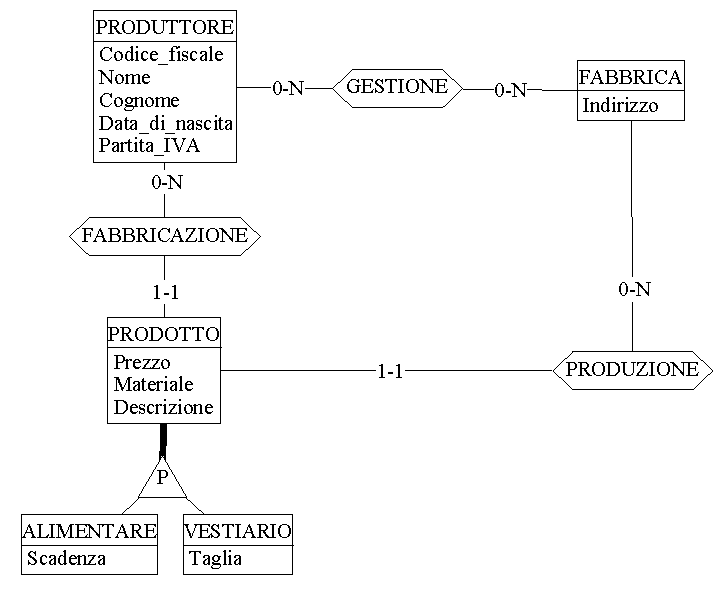
\includegraphics[width=\textwidth]{img/SchemaConcettuale-Produttori1.pdf}
	\caption{Schema scheletro per i Produttori}
\end{figure}
\subsection{Raffinamenti proposti}
Come per Corriere e Cliente, Produttore è estensione dell'entità generica Persona, che viene aggiunta. 
La relazione gestische tra Produttore e Fabbrica non è corretta, perchè non si riesce a mantenere uno storico dei diversi produttori di una fabbrica.
Perciò si decide di trasformarla in una entità, con attributi la data di inizio e la eventuale data di fine gestione della fabbrica. Viene collegata da relazioni 1-1 verso Produttore attraverso la relazione Gestione e con Amministrazione verso Fabbrica, e si mantiene 0-N nel verso opposto.
Per mantenere lo storico dei prezzi dei prodotti si crea un'entità Prodotto In Vendita, come nello schema Clienti.
Come identificatore di Produttore si usa quello di Persona, per Fabbrica e Prodotto si usa un codice. Prodotto in Vendita usa come identificatore quello importato da Prodotto più la data.
\subsection{Schema concettuale parziale}
\begin{figure}[H]
	\centering{}
	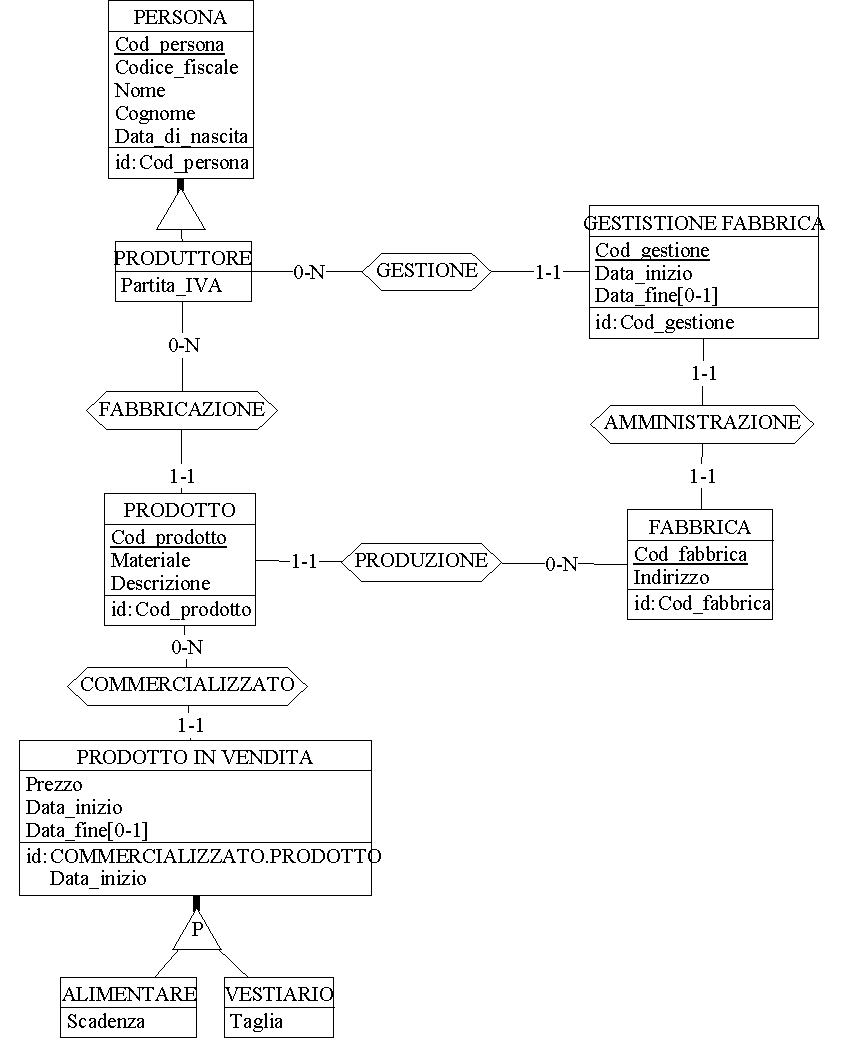
\includegraphics[width=\textwidth]{img/SchemaConcettuale-Produttori2.pdf}
	\caption{Schema scheletro per i Produttori, dopo le modifiche apportate}
\end{figure}
\section{Integrazione delle viste}
Nei seguenti schemi vengono mostrate solo le entità e relazioni che servono per unire le viste, per rendere migliore l'immagine. Lo schema finale completo è nella sezione successiva.
\subsection{Unione tra Corrieri e Clienti}
L'unione tra Corrieri e Clienti avviene in due entità. Sia Cliente che Corriere sono generalizzazioni di Persona, quindi vengono unite nella gerarchia totale ed esclusiva.
\begin{figure}[H]
	\centering{}
	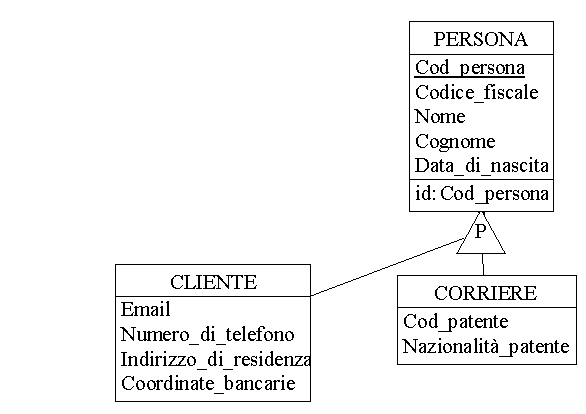
\includegraphics[width=\textwidth]{img/Unione-Clienti-Corrieri1.pdf}
	\caption{Unione di Corrieri e Clienti, via Persona}
\end{figure}
Un'altra unione degli schemi concettuali avviene in corrispondenza dell'entità Consegna, che è presente in entrambi gli schemi. 
\begin{figure}[H]
	\centering{}
	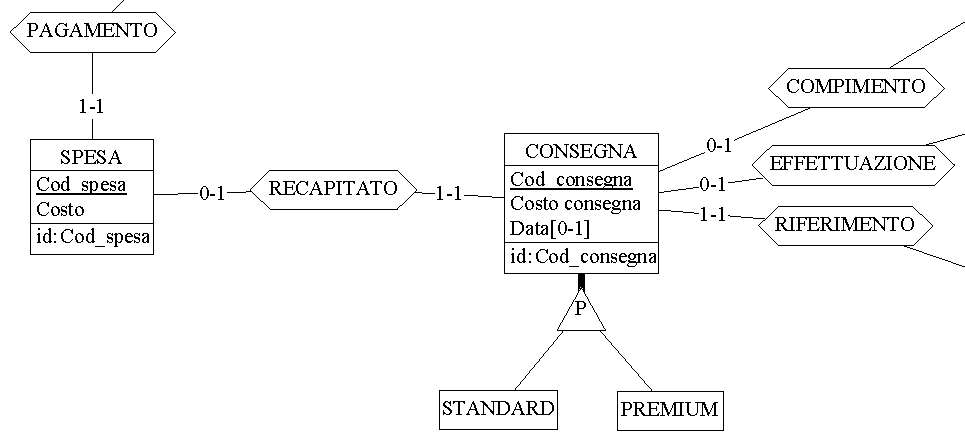
\includegraphics[width=\textwidth]{img/Unione-Clienti-Corrieri2.pdf}
	\caption{Unione di Corrieri e Clienti, via Consegna}
\end{figure}
\subsection{Unione tra Clienti e Produttori}

L'unione tra Produttori e Clienti avviene in due entità. Sia Cliente che Produttore sono generalizzazioni di Persona, quindi vengono unite nella gerarchia totale ed esclusiva. Nell'immagine compare anche Corrriere per l'unione degli schemi precedente.
\begin{figure}[H]
	\centering{}
	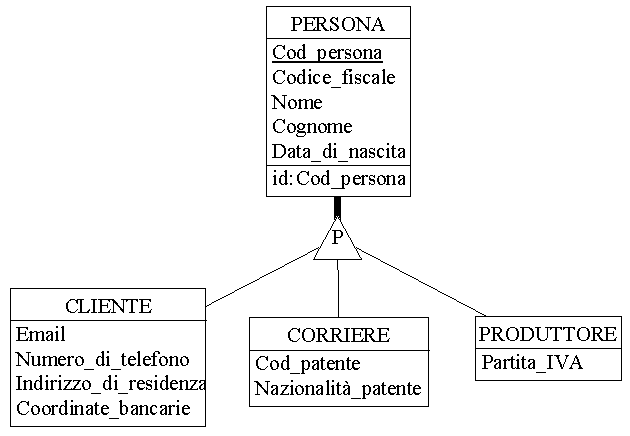
\includegraphics[width=\textwidth]{img/Unione-Clienti-Produttori1.pdf}
	\caption{Unione di Corrieri e Produttore, via Persona}
\end{figure}
Un'altra unione degli schemi concettuali avviene in corrispondenza dell'entità Prodotto e Prodotto in Vendita, che è presente in entrambi gli schemi. 
\begin{figure}[H]
	\centering{}
	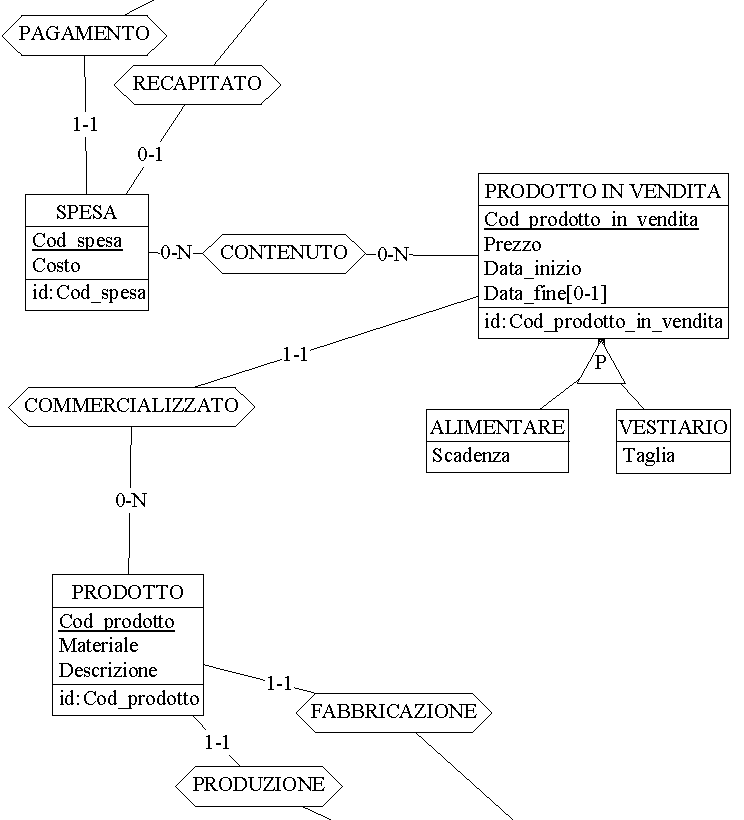
\includegraphics[width=\textwidth]{img/Unione-Clienti-Produttori2.pdf}
	\caption{Unione di Corrieri e Clienti, via Prodotto e Prodotto in Vendita}
\end{figure}

\section{Schema concettuale finale}
Lo schema concettuale finale, dopo l'integrazione delle viste:
\begin{figure}[h]
	\centering{}
	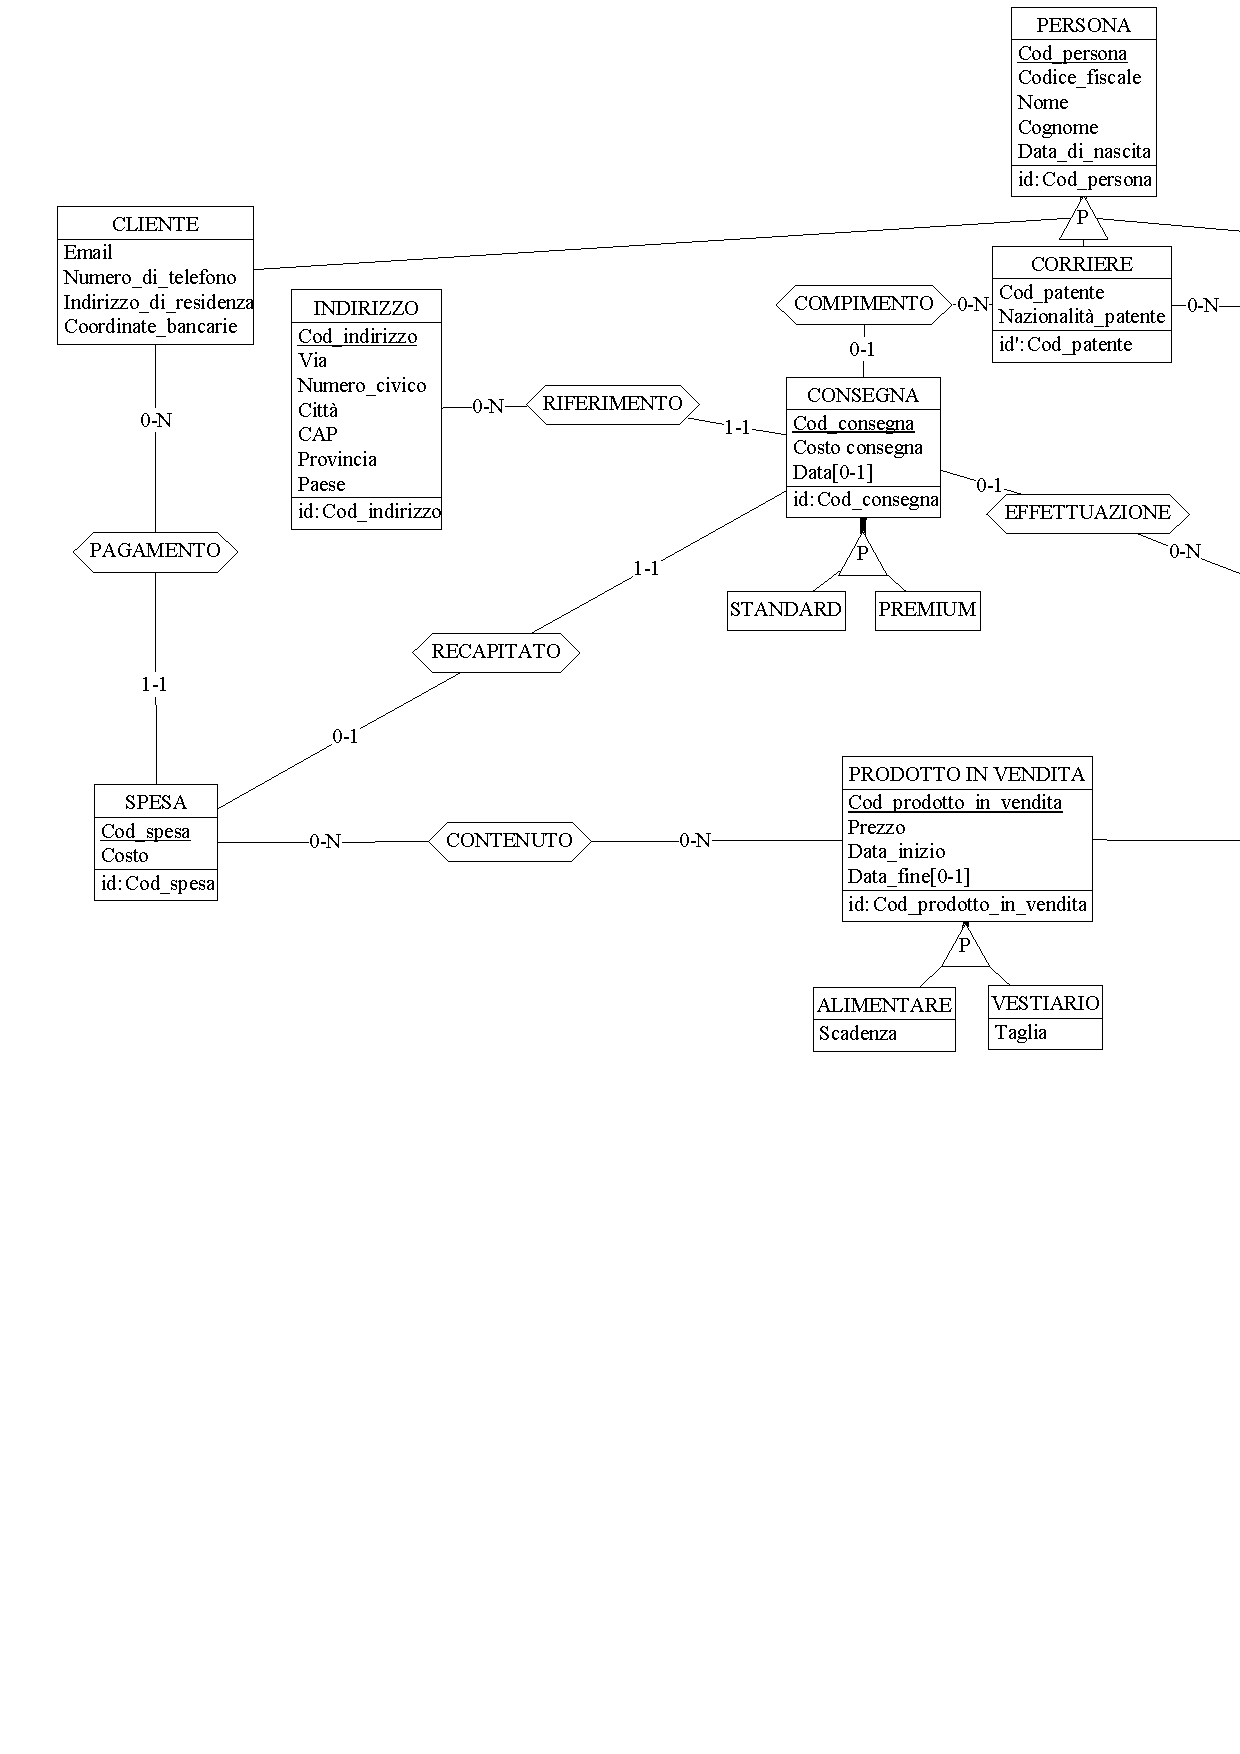
\includegraphics[width=\textwidth]{img/SchemaConcettuale-fin1.pdf}
	\caption{Lo schema concettuale finale, prima pagina}
\end{figure}
\begin{figure}[h]
	\centering{}
	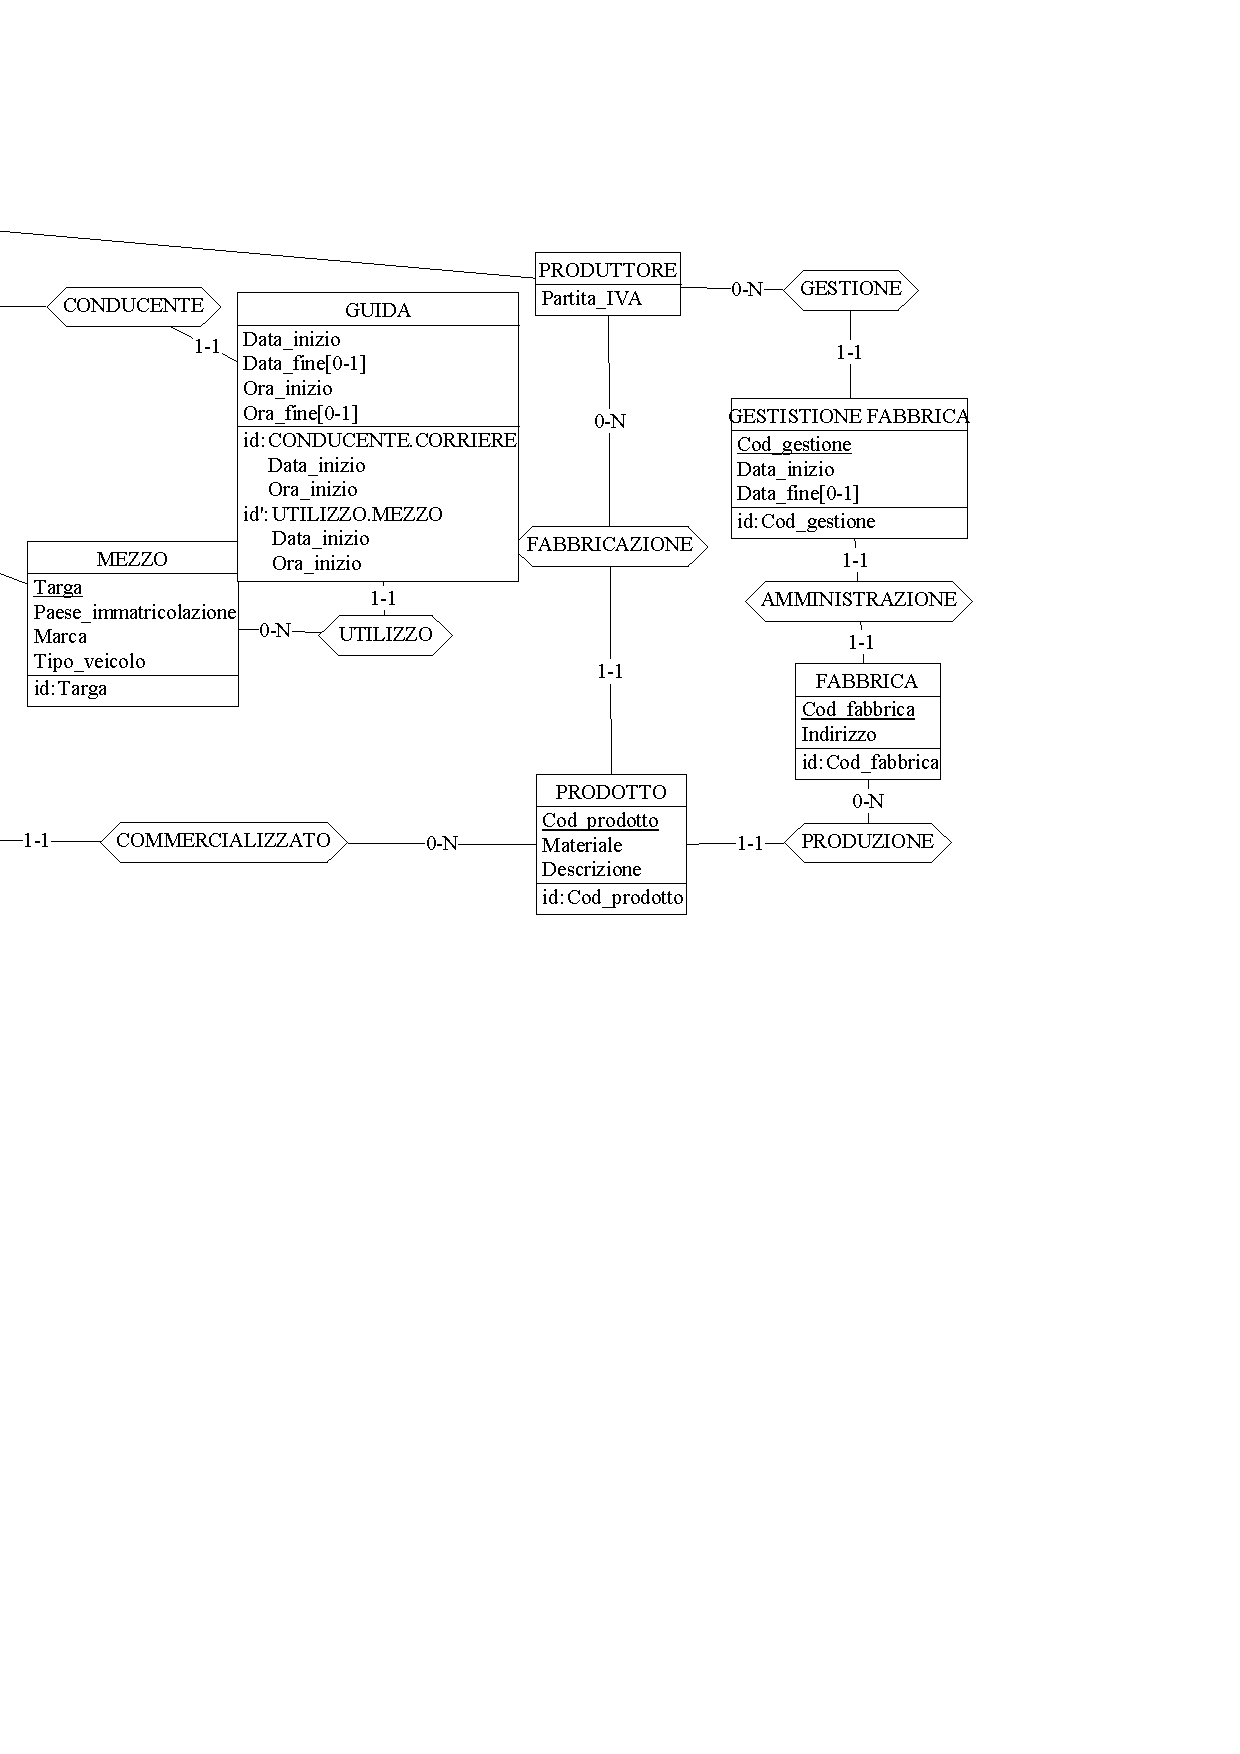
\includegraphics[width=0.50\textwidth]{img/SchemaConcettuale-fin2.pdf}
	\caption{Lo schema concettuale finale, seconda pagina}
\end{figure}
\chapter{Progettazione Logica}
\section{Stima del volume dei dati}
\begin{center}
    \begin{tabular}{ | c  c  c|} 
    \hline
    Concetto&Costrutto&Volume \\
    \hline
	\hline
    Cliente&E&10000 \\
	Spesa&E&50000 \\
	Pagamento&R&50000 \\
	\hline
	Prodotto in Vendita (Vestiario) &E&10000 \\
	Prodotto in Vendita (Alimentare) &E&20000 \\
	Contenuto&R&38000 \\
	Prodotto&E&10000 \\
	Commercializzato&R&30000 \\
	\hline
	Fabbrica&E&1000 \\
	Fabbricazione&R&3000 \\
	Gestione Fabbrica&E&2000 \\
	Amministrazione&R&1000 \\
	Produttore&E&800\\
	Gestione&R&2000 \\
	Produzione&R&3000\\
	\hline
	Corriere&E&2500\\
	Guida&E&10000\\
	Conducente&R&10000\\
	Mezzo&E&3000\\
	Utilizzo&R&10000\\
	Consegna (Standard) &E&35000\\
	Consegna (Premium) &E&15000\\
	Effettuazione&R&50000\\
	Utilizzo&R&2500\\
	Indirizzo&E&25000\\
	Riferimento&R&30000\\
	Recapitato&R&50000\\
	Compimento&R&50000\\
    \hline
    \end{tabular}
\end{center}
\section{Descrizione delle operazioni principali e stima della loro frequenza}
\begin{center}
    \begin{tabular}{ | c | c | c |} 
    \hline
    Codice&Operazione&Frequenza\\
    \hline
	1&Inserire un nuovo cliente&1000 al giorno\\
	\hline
	2&Cambiare il prezzo ad un prodotto esistente&100 al giorno\\
	\hline
	3&Creare una nuova guida ad un corriere ed un mezzo esistenti&200 al giorno\\
	\hline
	4&Leggere il prezzo medio di un prodotto&10 al giorno\\
	\hline
	5&Leggere quale corriere ha consegnato una data spesa&100 al giorno\\
	\hline
	6&Trovare il produttore di un dato prodotto&1000 al giorno\\
	\hline
	7&Creare una nuova spesa&100 al giorno\\
	\hline
	8&Leggere l'indirizzo associato ad una consegna&2000 al giorno\\
	\hline
	9&Cercare un prodotto di una taglia specifica&100 al giorno\\
	\hline 
	10&Cercare tutte le consegne di un corriere&20 al giorno\\
	\hline
	11&Ricavare l'ultima consegna ad un cliente&100 al giorno\\
	\hline
	12&Cambiare gestione ad una fabbrica&1 al giorno\\
	\hline
	13&Inserire un nuovo mezzo&2 al giorno\\
	\hline
    \end{tabular}
\end{center}
\section{Schemi di navigazione e tabelle degli accessi}
Sono riportate in seguito gli accessi necessarie per eseguire le operazioni riportate. 
Gli schemi di navigazione sono presenti solo per operazioni non banali. Per calcolare i costi si considera un accesso in scrittura come doppio rispetto a uno in lettura.\\
\textbf{Operazione 1:}
Iscrivere un nuovo Cliente
\begin{center}
    \begin{tabular}{ | c   c   c   c | } 
    \hline
    Concetto&Costrutto&Accessi&Tipo\\
	\hline
	Cliente&E&1&S\\
	\hline
	\end{tabular}
\end{center}
Totale: 1S → 2000 costo totale\\
\textbf{Operazione 2:}
Cambiare il prezzo ad un prodotto esistente
\begin{center}
    \begin{tabular}{ | c   c   c   c | } 
    \hline
    Concetto&Costrutto&Accessi&Tipo\\
	\hline
	Commercializzato&R&1&S\\
	\hline
	Prodotto in Vendita&E&1&S\\
	\hline
	\end{tabular}
\end{center}
Totale: 2S → 200 costo totale\\
\textbf{Operazione 3:}
Creare una nuova guida ad un corriere ed un mezzo esistenti
\begin{center}
    \begin{tabular}{ | c   c   c   c | } 	
    \hline
	Concetto&Costrutto&Accessi&Tipo\\
	\hline
	Guida&E&1&S\\
	\hline
	Conducente&R&1&S\\
	\hline
	Utilizzo&R&1&S\\
	\hline
	\end{tabular}
\end{center}
Totale: 3S → 600 costo totale\\
\textbf{Operazione 4:}
Leggere il prezzo medio di un prodotto\\
\begin{center}
    \begin{tabular}{ | c   c   c   c | } 
    \hline
	Concetto&Costrutto&Accessi&Tipo\\
	\hline
	Commercializzato&R&3&L\\
	\hline
    Prodotto in Vendita&E&3&L\\
	\hline
	\end{tabular}
\end{center}
Totale: 6L → 60 costo totale\\
\textbf{Operazione 5:}
Leggere quale corriere ha consegnato una data spesa\\
\begin{figure}[H]
	\centering{}
	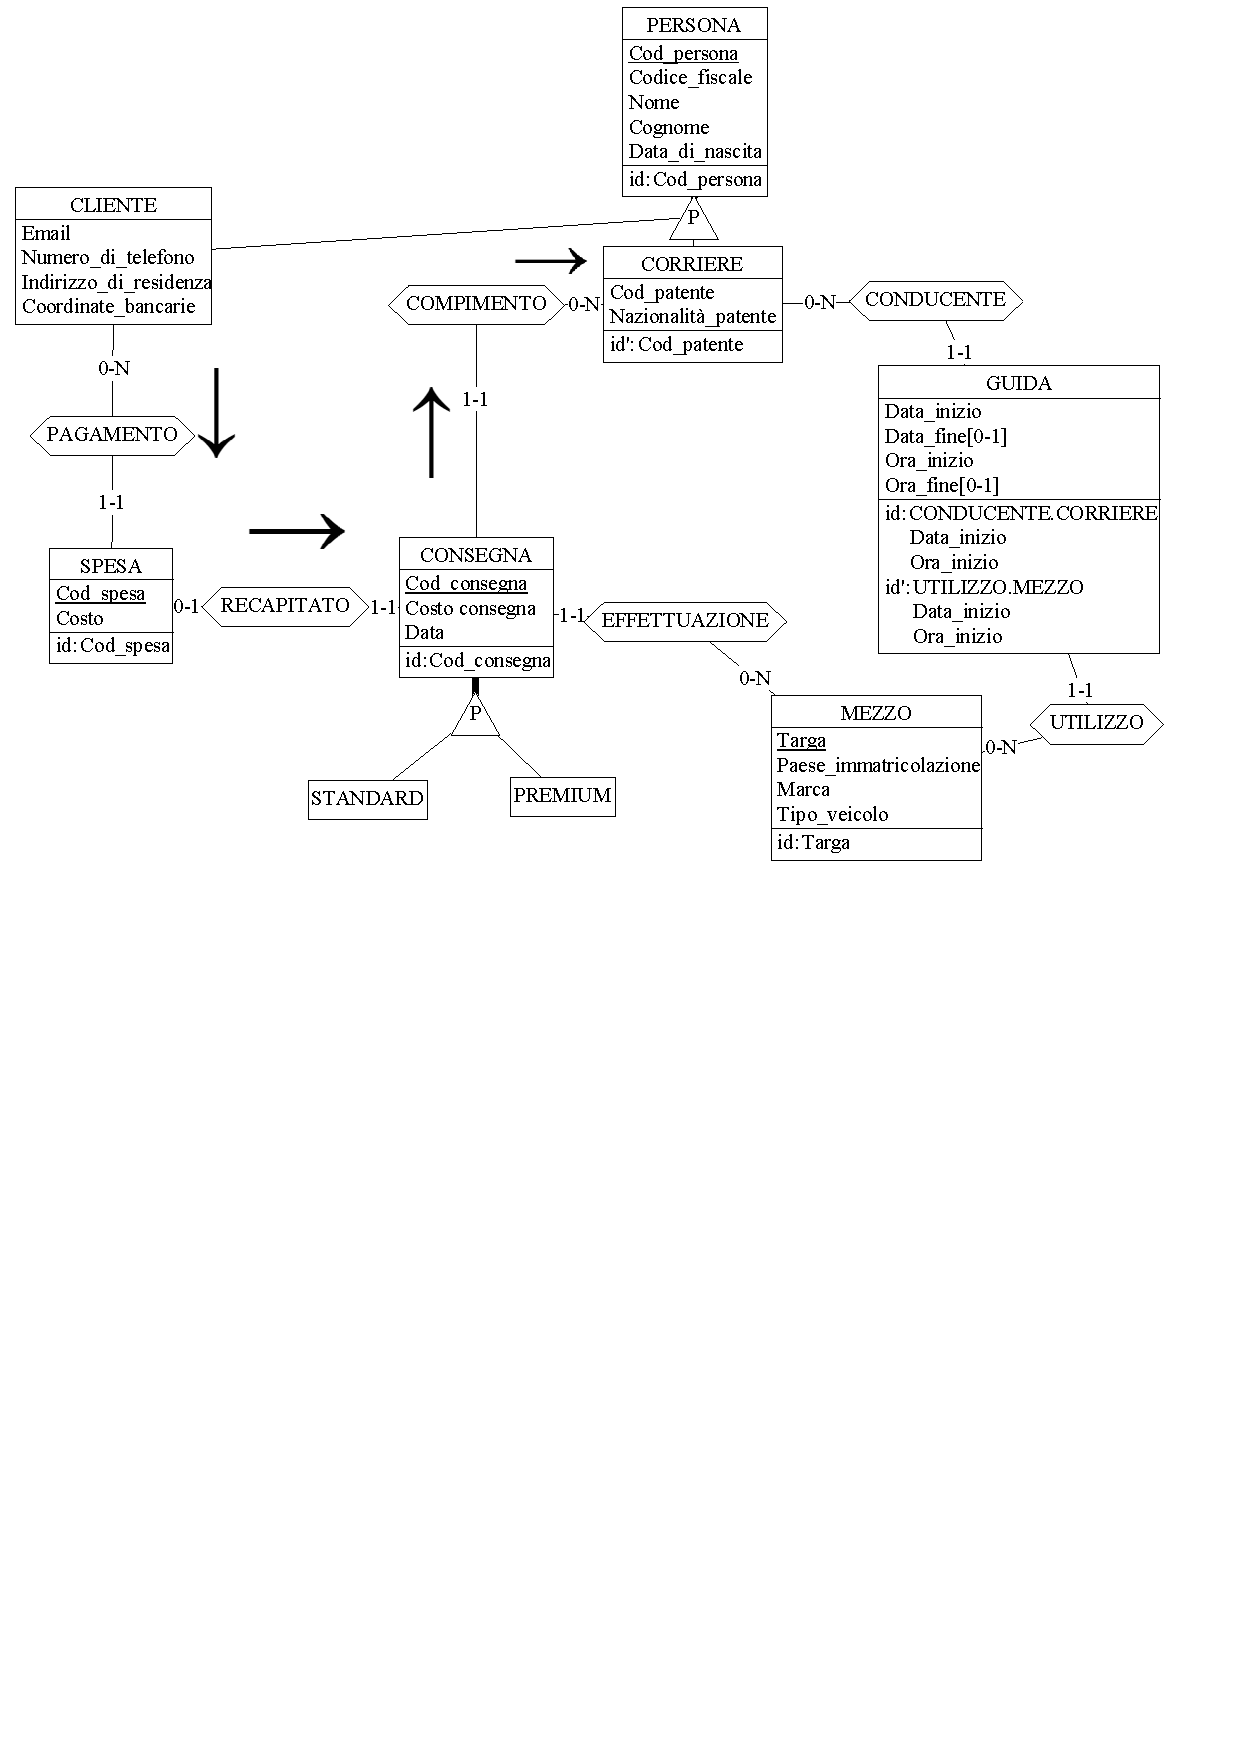
\includegraphics[width=\textwidth]{img/Operazione5.pdf}
	\caption{Si legge attraverso Consegna e Compimento i dati del corriere}
\end{figure}
\begin{center}
    \begin{tabular}{ | c   c   c   c | } 
    \hline
	Concetto&Costrutto&Accessi&Tipo\\
	\hline
	Recapitato&R&1&L\\
	\hline
    Consegna&E&1&L\\
	\hline
	Compimento&R&1&L\\
	\hline
	Corriere&E&1&L\\
	\hline
	\end{tabular}
\end{center}
Totale: 4L → 400 costo totale\\
\textbf{Operazione 6:}
Trovare il produttore di un dato prodotto\\
\begin{center}
    \begin{tabular}{ | c   c   c   c | } 
    \hline
	Concetto&Costrutto&Accessi&Tipo\\
	\hline
	Fabbricazione&R&1&L\\
	\hline
    Produttore&E&1&L\\
	\hline
	\end{tabular}
\end{center}
Totale: 2L → 2000 costo totale\\
\textbf{Operazione 7:}
Creare una nuova spesa\\
\begin{center}
    \begin{tabular}{ | c   c   c   c | } 
    \hline
	Concetto&Costrutto&Accessi&Tipo\\
	\hline
	Spesa&E&1&S\\
	\hline
	Pagamento&R&1&S\\
	\hline
	\end{tabular}
\end{center}
Totale: 2S → 400 costo totale\\
\textbf{Operazione 8:}
Leggere l'indirizzo associato ad una consegna\\
\begin{center}
    \begin{tabular}{ | c   c   c   c | } 
    \hline
	Concetto&Costrutto&Accessi&Tipo\\
	\hline
	Riferimento&R&1&L\\
	\hline
    Indirizzo&E&1&L\\
	\hline
	\end{tabular}
\end{center}
Totale: 2L → 4000 costo totale\\
\textbf{Operazione 9:}
Cercare un prodotto di una taglia specifica\\
\begin{center}
    \begin{tabular}{ | c   c   c   c | } 
    \hline
	Concetto&Costrutto&Accessi&Tipo\\
	\hline
	Commercializzato&R&3&L\\
	\hline
    Prodotto in Vendita&E&3&L\\
	\hline
	\end{tabular}
\end{center}
Totale: 6L → 600 costo totale\\

\textbf{Operazione 10:}
Cercare tutte le consegne di un corriere\\
\begin{center}
    \begin{tabular}{ | c   c   c   c | } 
    \hline
	Concetto&Costrutto&Accessi&Tipo\\
	\hline
	Compimento&R&20&L\\
	\hline
    Consegna&E&20&L\\
	\hline
	\end{tabular}
\end{center}
Totale: 40L → 800 costo totale\\
\textbf{Operazione 11:}
Ricavare l'ultima consegna ad un cliente\\
\begin{figure}[H]
	\centering{}
	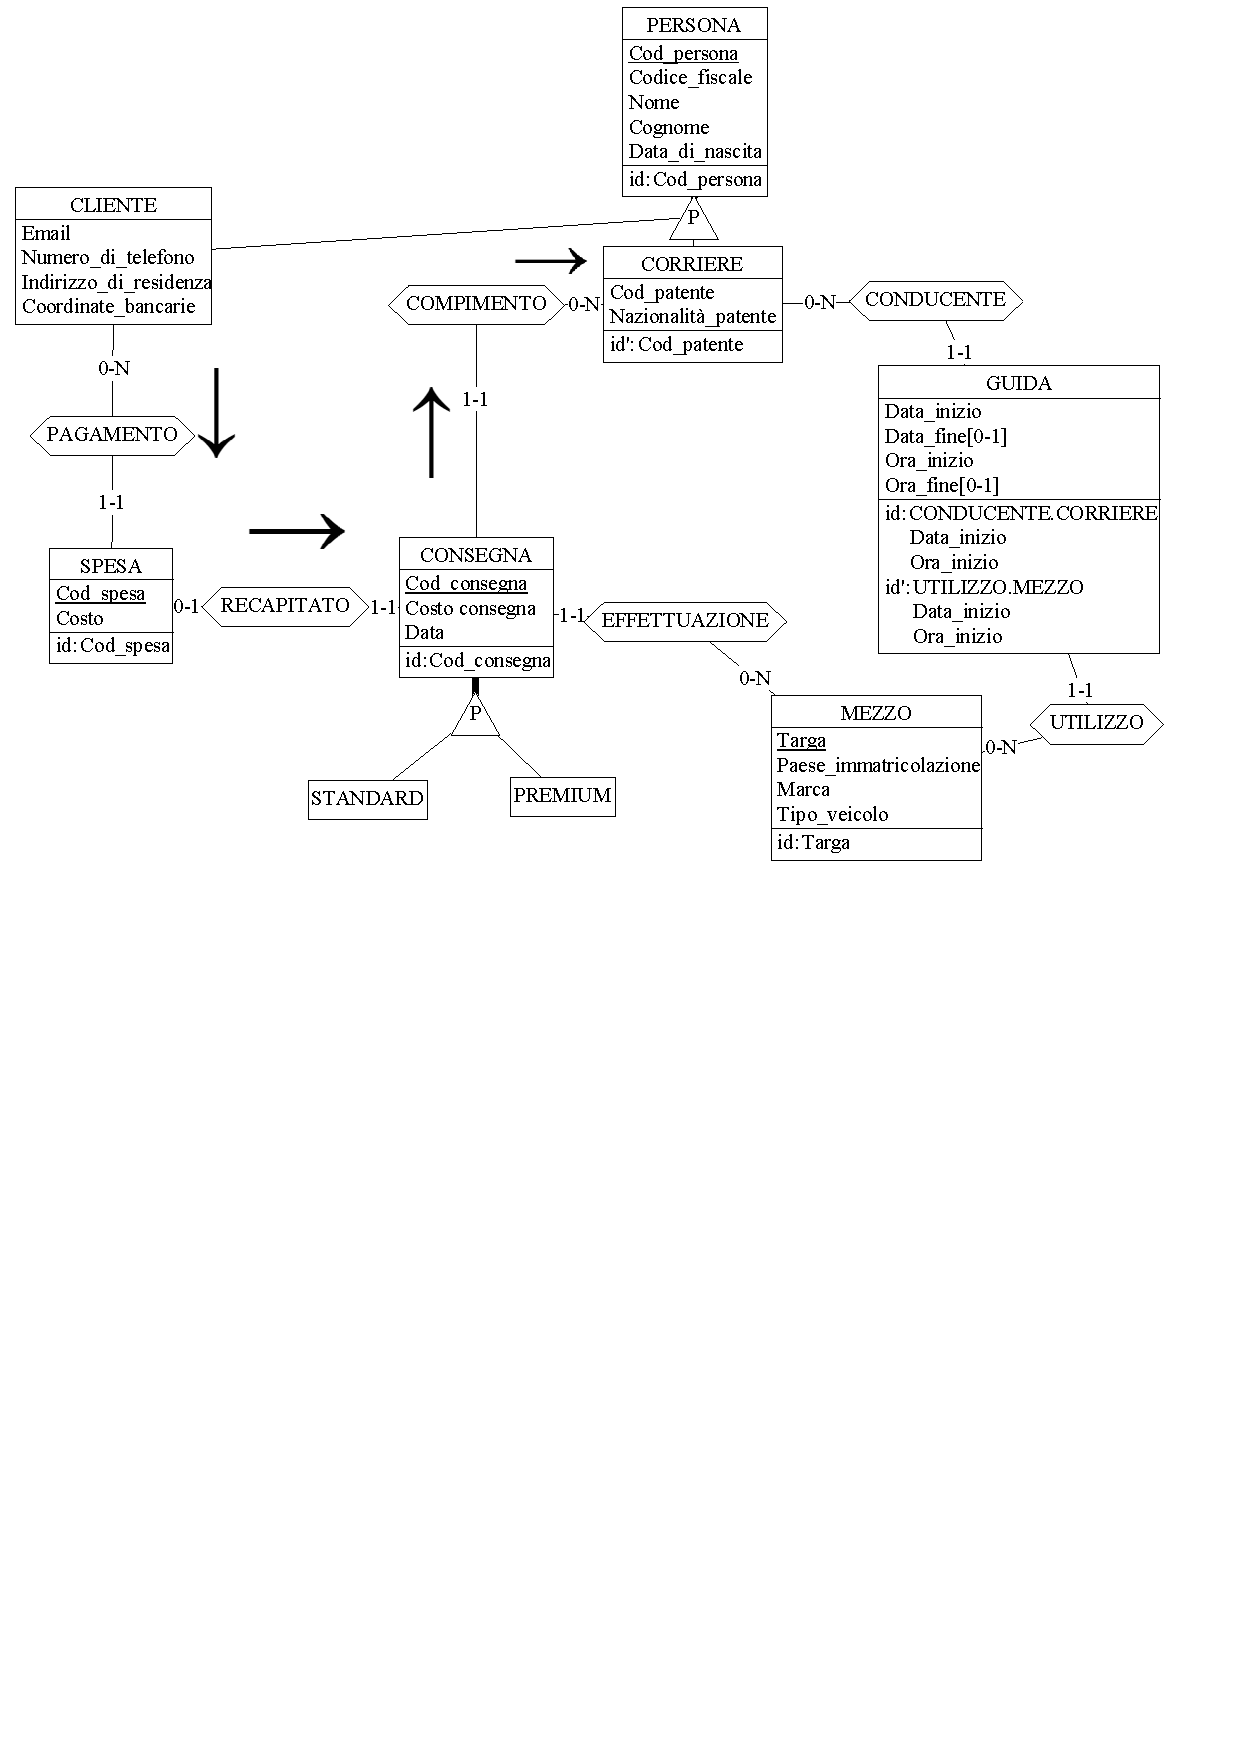
\includegraphics[width=\textwidth]{img/Operazione5.pdf}
	\caption{Si legge attraverso Pagamento e Spesa la data dell'ultima Consegna}
\end{figure}
\begin{center}
    \begin{tabular}{ | c   c   c   c | } 
    \hline
	Concetto&Costrutto&Accessi&Tipo\\
	\hline
	Pagamento&R&5&L\\
	\hline
    Spesa&E&5&L\\
	\hline
	Recapitato&R&5&L\\
	\hline
	Consegna&E&5&L\\
	\hline
	\end{tabular}
\end{center}
Totale: 20L → 2000 costo totale\\
\textbf{Operazione 12:}
Cambiare gestione ad una fabbrica\\
\begin{center}
    \begin{tabular}{ | c   c   c   c | } 
    \hline
	Concetto&Costrutto&Accessi&Tipo\\
	\hline
	Gestione&R&1&S\\
	\hline
    Gestione Fabbrica&E&1&S\\
	\hline
	Amministrazione&E&1&S\\
	\hline
	\end{tabular}
\end{center}
Totale: 3S → 6 costo totale\\
\textbf{Operazione 13:}
Inserire un nuovo mezzo\\
\begin{center}
    \begin{tabular}{ | c   c   c   c | } 
    \hline
	Concetto&Costrutto&Accessi&Tipo\\
	\hline
	Mezzo&E&1&S\\
	\hline
	\end{tabular}
\end{center}
Totale: 1S → 4 costo totale\\
\section{Raffinamento dello schema}
\subsection{Eliminazione delle gerarchie}
Nello schema ER compaiono tre gerarchie da eliminare.\\
Per lo schema di Persona, visto che la copertura è totale ed esclusiva e che l'entità Persona non è coinvolta in associazioni, si decide di effettuare un collasso verso il basso.
Come identificatori delle entità si rinomina Codice Persona in Codice Cliente in cliente, e così via nelle altre due entità.
\begin{figure}[H]
	\centering{}
	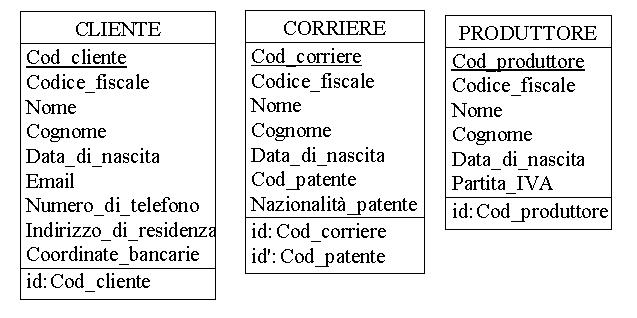
\includegraphics[width=\textwidth]{img/SchemaLogico-Persona.pdf}
	\caption{Il collasso della gerarchia di Persona}
\end{figure}
Per lo schema di Consegna per rimuovere la gerachia, effettuo un collasso verso l'alto, dato che le entità figlie non hanno relazioni e la copertura è totale ed esclusiva. 
Si introduce quindi in Consegna un attributo selettore, chiamato Tipo che assumerà due valori, Standard e Premium. 
\begin{figure}[H]
	\centering{}
	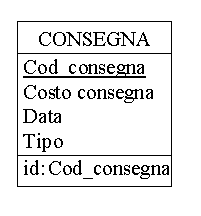
\includegraphics[width=\textwidth]{img/SchemaLogico-Consegna.pdf}
	\caption{Il collasso della gerarchia di Consegna}
\end{figure}
L'ultima gerarchia è quella di Prodotto In Vendita. Vista l'assenza di relazioni sulle entità figlie e la gerarchia totale ed esclusiva, effettuo un collasso verso l'alto. 
Prodotto In Vendita quindi avrà un attributo selettore chiamato Tipo, che avrà due valori, Vestiario e Alimentare. Inoltre vengono aggiunti due attributi opzionali Taglia e Scadenza.
\begin{figure}[H]
	\centering{}
	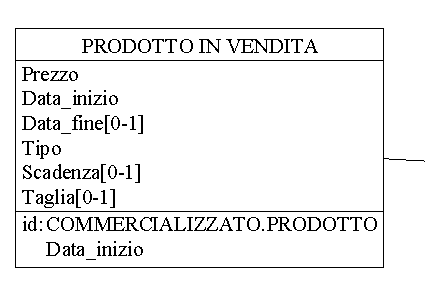
\includegraphics[width=\textwidth]{img/SchemaLogico-Prodotto.pdf}
	\caption{Il collasso della gerarchia di Prodotto}
\end{figure}
\subsection{Eliminazione degli attributi composti}
L'unico attributo composto presente nello schema concettuale è Indirizzo, presente nelle entità Cliente e Fabbrica. Viene suddiviso in tre attributi: Via, Numero Civico, Città in ognuna delle entità.
\subsection{Scelta delle chiavi primarie}
Le chiavi primarie scelte sono presenti nello schema concettuale finale. 
L'unica modifica è la creazione di un Codice Guida, che permette di identificare più facilmente la Guida.
\subsection{Eliminazione degli identificatori esterni}
Nello schema ER sono state eliminate le seguenti relazioni:\\
Pagamento viene rimosso, Spesa incorpora il codice persona di cliente\\
Recapitato viene rimosso, Consegna incorpora il codice Spesa (opzionale)\\
Contenuto diventa una entità, con come attributi il codice spesa e codice prodotto in vendita, che formano la chiave primaria \\
Compimento viene rimosso, Consegna incorpora il codice persona di corriere (opzionale)\\
Effettuazione viene rimosso, Consegna incorpora la targa (opzionale)\\
Riferimento viene rimosso, Consegna incorpora il codice indirizzo\\
Conducente viene rimosso, Guida incorpora il codice persona di corriere\\
Utilizzo viene rimosso, Guida incorpora la targa\\
Commercializzato viene rimosso, Prodotto in Vendita incorpora il codice prodotto\\
Fabbricazione viene rimosso, Prodotto incorpora il codice persona di produttore\\
Gestione viene rimosso, Gestione fabbriche incorpora il codice persona di produttore\\
Amministrazione viene rimosso, Gestione fabbriche incorpora il codice fabbrica\\
Produzione viene rimosso, Prodotto incorpora il codice prodotto\\
\section{Analisi delle ridondanze}
Ci sono due relazioni ridondanti nello schema concettuale: Compimento e Fabbricazione.
\subsection{Analisi delle ridondanze: Compimento}
\textbf{Con ridondanza:}\\
\textbf{Operazione 5:}Leggere quale corriere ha consegnato una data spesa\\
\begin{center}
    \begin{tabular}{ | c   c   c   c | } 
    \hline
	Concetto&Costrutto&Accessi&Tipo\\
	\hline
	Recapitato&R&1&L\\
	\hline
    Consegna&E&1&L\\
	\hline
	Compimento&R&1&L\\
	\hline
	Corriere&E&1&L\\
	\hline
	\end{tabular}
\end{center}
Totale: 4L → 400 costo totale\\
\textbf{Operazione 10:}
Cercare tutte le consegne di un corriere\\
\begin{center}
    \begin{tabular}{ | c   c   c   c | } 
    \hline
	Concetto&Costrutto&Accessi&Tipo\\
	\hline
	Compimento&R&20&L\\
	\hline
    Consegna&E&20&L\\
	\hline
	\end{tabular}
\end{center}
Totale: 40L → 800 costo totale\\
\textbf{Senza ridondanza:}\\
\textbf{Operazione 5:}Leggere quale corriere ha consegnato una data spesa\\
\begin{center}
    \begin{tabular}{ | c   c   c   c | } 
    \hline
	Concetto&Costrutto&Accessi&Tipo\\
	\hline
	Recapitato&R&1&L\\
	\hline
    Consegna&E&1&L\\
	\hline
	Effettuazione&R&1&L\\
	\hline
	Mezzo&E&1&L\\
	\hline
	Utilizzo&R&4&L\\
	\hline
	Guida&E&4&L\\
	\hline
	Conducente&R&4&L\\
	\hline
	Corriere&E&4&L\\
	\hline
	\end{tabular}
\end{center}
Totale: 20L → 2000 costo totale\\
\textbf{Operazione 10:}
Cercare tutte le consegne di un corriere\\
\begin{center}
    \begin{tabular}{ | c   c   c   c | } 
    \hline
	Concetto&Costrutto&Accessi&Tipo\\
	\hline
	Conducente&R&4&L\\
	\hline
	Guida&E&4&L\\
	\hline
	Utilizzo&R&4&L\\
	\hline
	Mezzo&E&4&L\\
	\hline
	Effettuazione&R&17*4=68&L\\
	\hline
    Consegna&E&17*4=68&L\\
	\hline
	\end{tabular}
\end{center}
Totale: 152L → 3040 costo totale\\
\\
In totale mantenere la ridondanza ha un costo di 400+800=1200 operazioni al giorno, mentre rimuoverla ha un costo di 2000+3040=5040 operazioni al giorno. Si ha un evidente vantaggio computazionale a mantenere la ridondanza.\\
\subsection{Analisi delle ridondanze: Fabbricazione}
\textbf{Con ridondanza:}\\
\textbf{Operazione 6:} Trovare il produttore di un dato prodotto\\
\begin{center}
    \begin{tabular}{ | c   c   c   c | } 
    \hline
	Concetto&Costrutto&Accessi&Tipo\\
	\hline
	Fabbricazione&R&1&L\\
	\hline
    Produttore&E&1&L\\
	\hline
	\end{tabular}
\end{center}
Totale: 2L → 2000 costo totale\\
\textbf{Senza ridondanza:}\\
\textbf{Operazione 6:} Trovare il produttore di un dato prodotto\\
\begin{center}
    \begin{tabular}{ | c   c   c   c | } 
    \hline
	Concetto&Costrutto&Accessi&Tipo\\
	\hline
	Produzione&R&1&L\\
	\hline
	Fabbrica&E&1&L\\
	\hline
	Amministrazione&R&1&L\\
	\hline
	Gestione Fabbrica&E&1&L\\
	\hline
	Gestione&R&1&L\\
	\hline
    Produttore&E&1&L\\
	\hline
	\end{tabular}
\end{center}
Totale: 6L → 6000 costo totale\\
\\
In totale mantenere la ridondanza ha un costo di 2000 operazioni al giorno, mentre rimuoverla ha un costo di 6000 operazioni al giorno. Si ha un evidente vantaggio computazionale a mantenere la ridondanza.\\
\section{Traduzione di entità e associazioni in relazioni}
Cliente(\underline{Cod\_cliente}, Codice\_fiscale, Nome, Cognome, Data\_di\_nascita, Email, Numero\_di\_telefono, Via\_residenza, Numero\_civ\_residenza, Città\_residenza, Coordinate\_bancarie)\\
Spesa(\underline{Cod\_spesa}, Costo, Cod\_cliente: Cliente)\\
Contenuto(\underline{Cod\_spesa: Spesa, Cod\_prodotto\_vendita: Prodotto in Vendita})\\
Prodotto In Vendita(\underline{Cod\_prodotto\_vendita}, Prezzo, Data\_inizio, Data\_fine*, Tipo, Scadenza*, Taglia*, Cod\_Prodotto: Prodotto)\\
Prodotto(\underline{Cod\_prodotto}, Materiale, Descrizione, Cod\_produttore: Produtore, Cod\_fabbrica: Fabbrica)\\
Fabbrica(\underline{Cod\_fabbrica}, Via, Numero\_civ, Città)\\
Gestione Fabbrica(\underline{Cod\_gestione}, Cod\_fabbrica: Fabbrica, Data\_inizio, Data\_fine*, Cod\_produttore: Produttore)\\
Produttore(\underline{Cod\_produttore}, Codice\_fiscale, Nome, Cognome, Data\_di\_nascita, Partita\_IVA)\\
Consegna(\underline{Cod\_consegna}, Cod\_spesa*:Spesa, Costo\_consegna, Data, Tipo, Cod\_indirizzo: Indirizzo, Cod\_corriere: Corriere, Targa: Mezzo)\\
Indirizzo(\underline{Cod\_indirizzo}, Via, Numero\_civico, Città, CAP, Provincia, Paese)\\
Corriere(\underline{Cod\_corriere}, Codice\_fiscale, Nome, Cognome, Data\_di\_nascita, Cod\_patente, Nazionalità\_patente)\\
Mezzo(\underline{Targa}, Paese\_immatricolazione, Marca, Tipo\_Veicolo)\\
Guida(\underline{Cod\_guida}, Data\_inizio, Data\_fine*, Ora\_inizio, Ora\_fine*, Cod\_corriere: Corriere, Targa: Mezzo)\\
\section{Schema relazionale finale}
\begin{figure}[H]
	\centering{}
	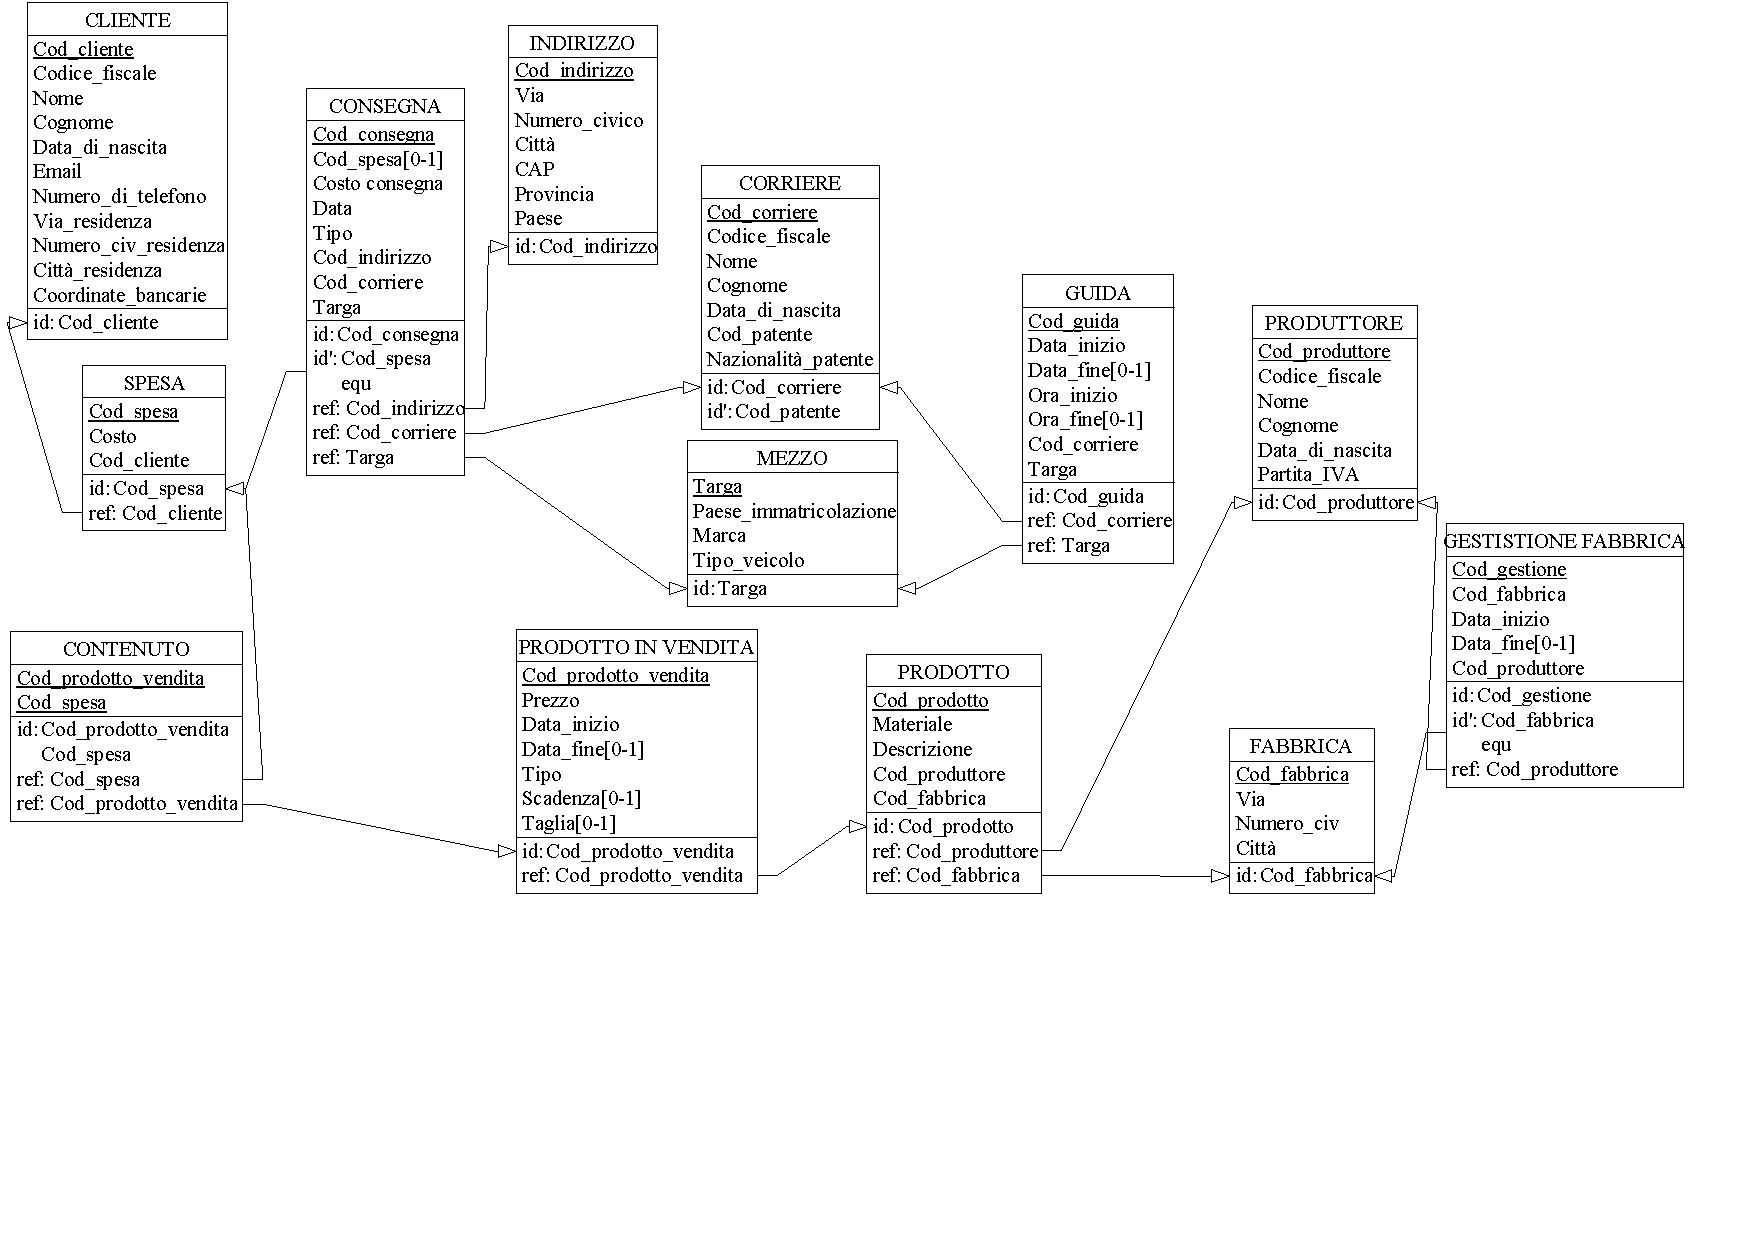
\includegraphics[width=\textwidth]{img/SchemaLogico-fin.pdf}
	\caption{Lo schema logico finale}
\end{figure}
\section{Traduzione delle operazioni in query SQL}
\textbf{Operazione 1:}
Iscrivere un nuovo Cliente\\
INSERT INTO CLIENTI (Codice\_fiscale, Nome, Cognome, Data\_di\_nascita, Email, Numero\_di\_telefono, Via\_residenza, Numero\_civ\_residenza, Città\_residenza, Coordinate\_bancarie)\\
VALUES ('?','?','?','?', '?', ?, '?', ?, '?', '?');\\
\textbf{Operazione 2:}
Cambiare il prezzo ad un prodotto esistente\\
INSERT INTO PRODOTTI\_IN\_VENDITA(Prezzo, Data\_inizio, Tipo, Scadenza, Taglia, Cod\_prodotto)\\
VALUES (?, '?', 'Vestiario/Alimentare', '?', '?', ?);\\
\textbf{Operazione 3:}
Creare una nuova guida ad un corriere ed un mezzo esistenti\\
INSERT INTO GUIDE(Data\_inizio, Data\_fine, Ora\_inizio, Ora\_fine, Cod\_corriere, Targa)\\
VALUES('?', '?', ?, ?, ?, '?');\\
\textbf{Operazione 4:}
Leggere il prezzo medio di un prodotto\\
SELECT avg(Prezzo) as Prezzo\_medio\\
FROM PRODOTTI\_IN\_VENDITA, PRODOTTI\\
WHERE PRODOTTI\_IN\_VENDITA.Cod\_prodotto=PRODOTTI.Cod\_prodotto AND PRODOTTI.Cod\_Prodotto='?';\\
\textbf{Operazione 5:}
Leggere quale corriere ha consegnato una data spesa\\
SELECT corr.Nome, corr.Cognome, corr.Cod\_corriere\\
FROM SPESE s, CONSEGNE c, CORRIERI corr\\
WHERE c.Cod\_spesa=s.Cod\_spesa AND c.Cod\_corriere=corr.Cod\_corriere AND s.Cod\_spesa='?';\\
\textbf{Operazione 6:}
Trovare il produttore di un dato prodotto\\
SELECT PRODUTTORI.Nome, PRODUTTORI.Cognome, PRODUTTORI.Cod\_produttore\\
FROM PRODUTTORI, PRODOTTI\\
WHERE PRODOTTI.Cod\_produttore=PRODUTTORI.Cod\_produttore AND Cod\_prodotto='?';\\
\textbf{Operazione 7:}
Creare una nuova spesa\\
INSERT INTO SPESE (Costo, Cod\_cliente)\\
VALUES (?,?);\\
\textbf{Operazione 8:}
Leggere l'indirizzo associato ad una consegna\\
SELECT i.Via, i.Numero\_civico, i.Città\\
FROM CONSEGNE c, INDIRIZZI i\\
WHERE c.Cod\_indirizzo=i.Cod\_indirizzo and c.Cod\_consegna=?;\\
\textbf{Operazione 9:}
Cercare un prodotto di una taglia specifica\\
SELECT pv.Prezzo, pv.Cod\_prodotto\_vendita, pv.Data\_inizio, pv.Data\_fine\\
FROM PRODOTTI p, PRODOTTI\_IN\_VENDITA pv\\
WHERE pv.Cod\_prodotto=p.Cod\_prodotto AND p.Cod\_prodotto=4 AND pv.Taglia='?' ;\\
\textbf{Operazione 10:}
Cercare tutte le consegne di un corriere\\
SELECT c.Cod\_consegna\\
FROM CONSEGNE c, CORRIERI cc\\
WHERE c.Cod\_corriere=cc.Cod\_corriere AND cc.Cod\_corriere='?';\\
\textbf{Operazione 11:}
Ricavare l'ultima consegna ad un cliente\\
SELECT c.Data\\
FROM CONSEGNE c, CORRIERI cc\\
WHERE c.Cod\_corriere=cc.Cod\_corriere AND cc.Cod\_corriere='?'\\
ORDER BY c.Data DESC LIMIT 1;\\
\textbf{Operazione 12:}
Cambiare gestione ad una fabbrica\\
INSERT INTO GESTIONE\_FABBRICHE (Cod\_fabbrica, Data\_inizio, Data\_fine, Cod\_produttore)\\
VALUES (?,'?', '?', ?);\\
\textbf{Operazione 13:}
Inserire un nuovo mezzo\\
INSERT INTO MEZZI(Targa, Paese\_immatricolazione, Marca, Tipo\_veicolo)\\
VALUES('?', '?', '?', '?');\\
\chapter{Progettazione dell'applicazione}
\section{Descrizione dell'architettura dell'applicazione}
L'applicazione per interfacciarsi con il Database è stata realizzata in linguaggio Java che rende possibile l'esecuzione di operazioni per l'utente. 
L'interfacciamento versio il Database è stato fornito da JDBC, il database risiede in locale e e usa MySQL come DBMS. 
L'applicazione usa JavaFX per la grafica, caricandola da file FXML, uno per ogni schermata che si appoggiano al loro Controller relativo. 
L'interazione con il database è stata gestita attraverso classi che estendono l'interfaccia Table, una per tabella del DB. 
Nel Model esistono classi che rappresentano il tipo di dato della tabella. Per il collegamento effettivo verso il database si usa una classe ConnectionProvider che ha il compito di creare la connessione.
\\
All'avvio dell'applicazione viene mostrata una schermata dove si chiedono le credenziali di mySQL, per accedere al database se necessario oppure per crearlo, se non è esistente.
\begin{figure}[H]
	\centering{}
	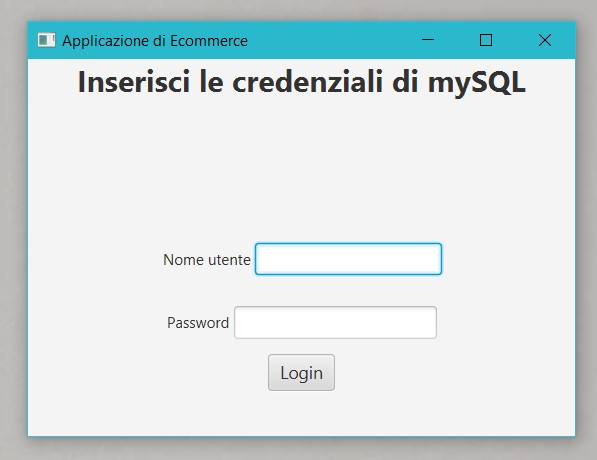
\includegraphics[width=\textwidth]{img/Application/Credentials.jpg}
	\caption{Il login con le credenziali di MySQL}
\end{figure}
Una volta acceduto compare una schermata di login, per permettere ai diversi utenti di identificarsi e fare operazioni diverse.
Attualmente per fare il login il nome utente è il codice dell'utente e la password il nome, ma in una fase successiva del progetto questo login verrà reso più sicuro, memorizzando una password (non in chiaro) e un nome utente. 
Il login permette di identificare univocamente quale utente esegue certe azioni e modificare il database di conseguenza. Il login va a buon fine solo se le credenziali sono uguali a quelle memorizzate nel database.
\subsection*{Schermate cliente}
Il cliente una volta entrato nell'applicazione dopo il login si trova in una schermata dove può visualizzare lo 
storico delle spese passate, assieme allo stato di consegna. Se il cliente ha delle spese non ancora consegnate può andare a vedere nel dettaglio l'indirizzo e altri dati.
\begin{figure}[H]
	\centering{}
	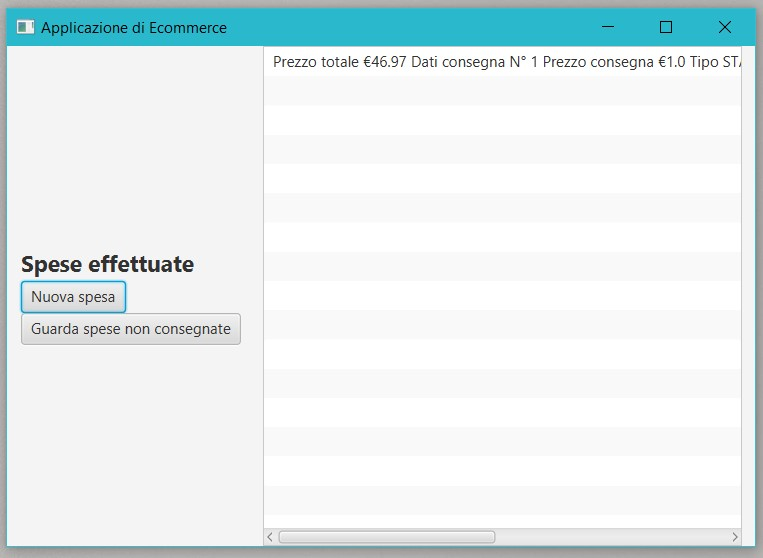
\includegraphics[width=\textwidth]{img/Application/ClientMenu1.jpg}
	\caption{La schermata iniziale per il cliente}
\end{figure}
Dalla schermata iniziale premendo il pulsante per creare una nuova spesa si passa alla selezione degli articoli da mettere nel carrello. 
Qui si possono filtrare gli elementi in vendita secondo due criteri distinti, o per taglia o per scadenza, a seconda del tipo dei prodotti.
\begin{figure}[H]
	\centering{}
	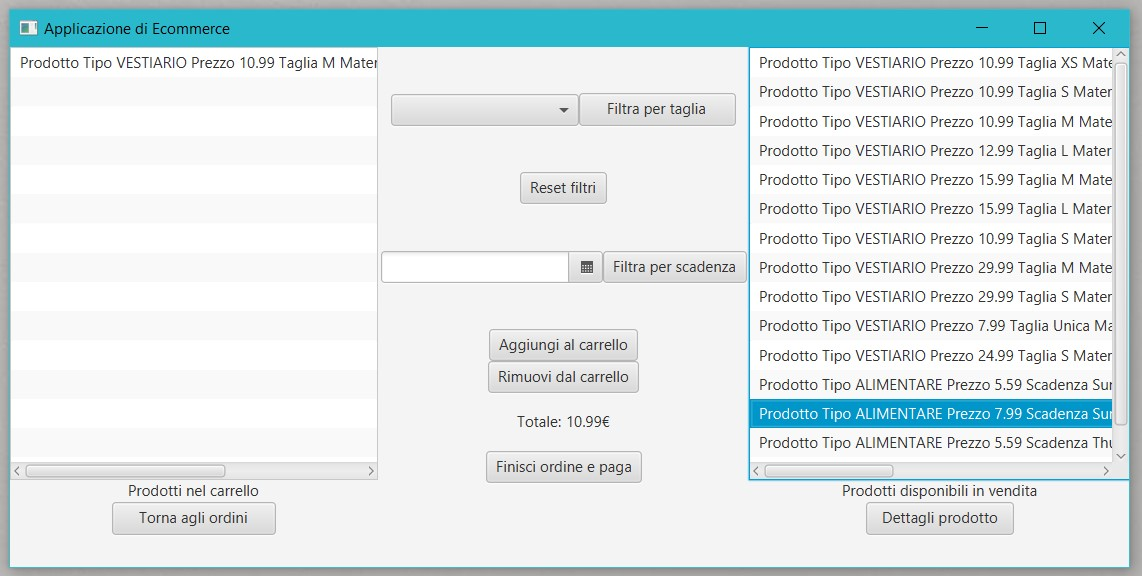
\includegraphics[width=\textwidth]{img/Application/ClientMenu2.jpg}
	\caption{La vista della creazione di una nuova spesa, con alcuni elementi nel carrello}
\end{figure}
Una volta che si ha un prodotto selezionato si possono andare a vedere i dettagli della produzione, come lo stabilimento produttivo oppure il produttore.
\begin{figure}[H]
	\centering{}
	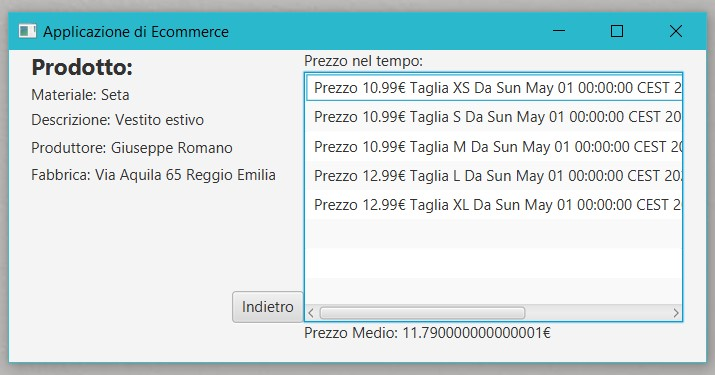
\includegraphics[width=\textwidth]{img/Application/ClientMenu3.jpg}
	\caption{I dettagli della produzione di un prodotto, come il prezzo medio e le versioni esisenti}
\end{figure}
Se si prosegue e si arriva alla schermata del pagamento, si può scegliere un indirizzo a cui 
farsi consegnare la spesa tra quelli usati in precedenza, altrimenti se ne può creare uno nuovo. 
Una volta selezionato l'indirizzo e il tipo di consegna desiderata si puo completare il pagamento, 
e se va a buon fine un messaggio comparirà a schermo dicendo il numero identificativo della spesa e si torna alla schermata iniziale del cliente.
\begin{figure}[H]
	\centering{}
	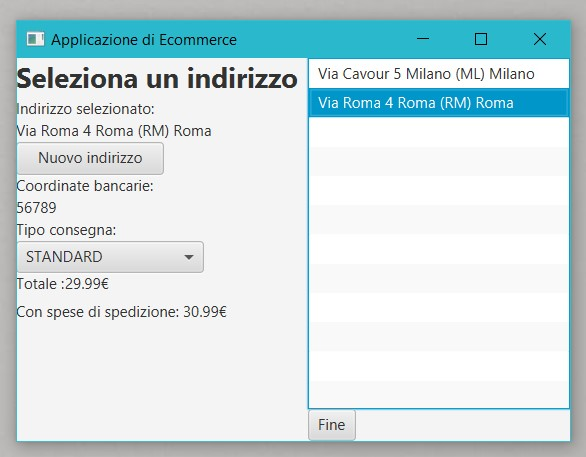
\includegraphics[width=\textwidth]{img/Application/ClientMenu4.jpg}
	\caption{La pagina dove si conclude la spesa, scegliendo l'indirizzo, il tipo di consegna e effettuando il pagamento}
\end{figure}

\subsection*{Schermate corriere}
Il corriere parte da una schermata dove vengono mostrate le consegne effettuate precedentemente, con la possibilità di guardare i dettagli delle consegne svolte.
Quando si va a creare una nuova consegna, il corriere sceglie tra le guide effettuate tra cui associare la consegna. 
Una volta effettuata la consegna, l'applicazione torna alla schermata iniziale.
\begin{figure}[H]
	\centering{}
	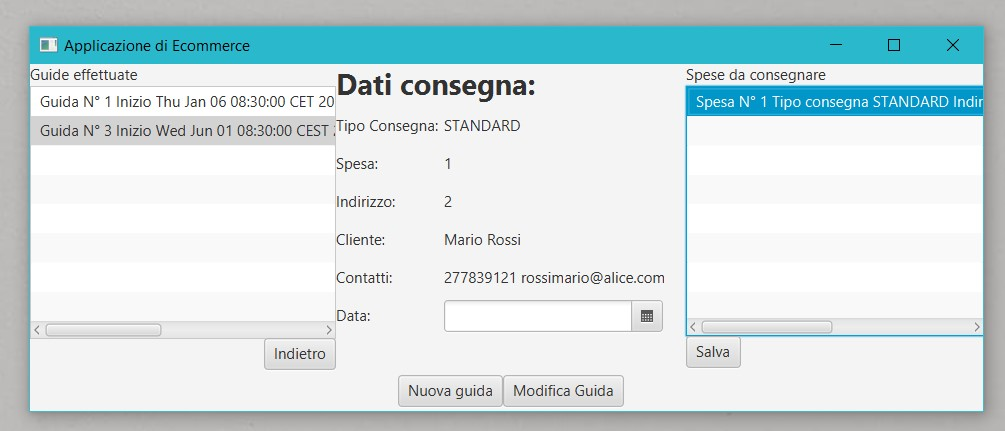
\includegraphics[width=\textwidth]{img/Application/Courier1.jpg}
	\caption{Associazione tra consegna e guida}
\end{figure}
Se la guida corretta non è presente si può crearla e una volta scelto un periodo svolgimento si può cercare un veicolo libero da associare. 
La nuova guida può essere creata solo se il corriere non è impegnato in altre guide nel periodo prescelto ed esistono mezzi liberi.
\begin{figure}[H]
	\centering{}
	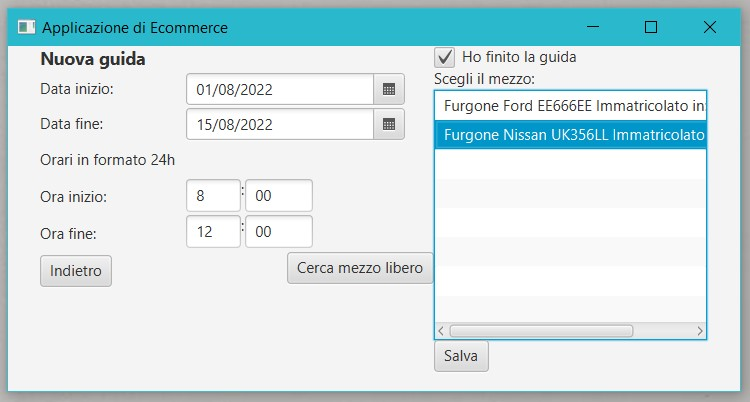
\includegraphics[width=\textwidth]{img/Application/Courier2.jpg}
	\caption{Creazione di una nuova guida}
\end{figure}
\subsection*{Schermate produttore}
La pagina iniziale per un produttore è una vista globale dei prodotti creati nelle fabbriche attualmente gestite. 
Si può decidere cambiare la messa in vendita di un prodotto, ad esempio creando una nuova taglia oppure creare un prodotto completamente nuovo.
\begin{figure}[H]
	\centering{}
	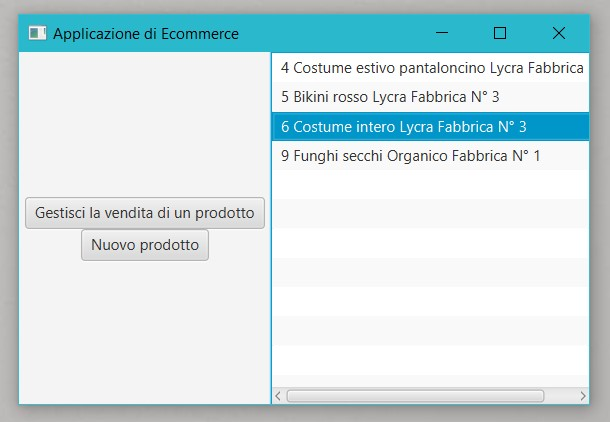
\includegraphics[width=\textwidth]{img/Application/Producer1.jpg}
	\caption{Pagina iniziale produttore}
\end{figure}
Quando si crea una nuova versione del prodotto, si specifica un prezzo, un periodo di vendita del prodotto e l'eventuale taglia o scadenza.
\begin{figure}[H]
	\centering{}
	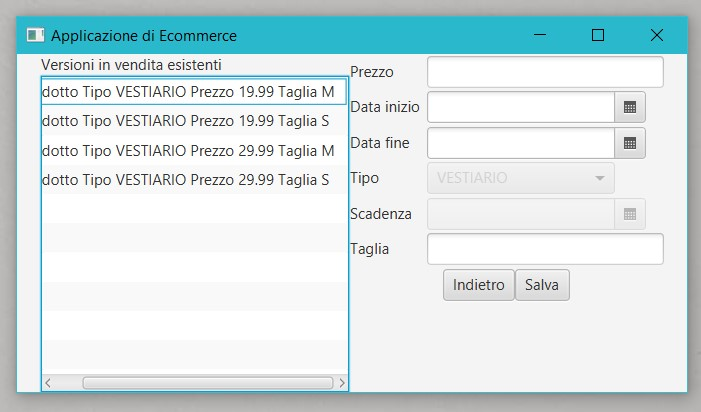
\includegraphics[width=\textwidth]{img/Application/Producer2.jpg}
	\caption{Creazione di una nuova versione del prodotto}
\end{figure}
Nella creazione di un nuovo prodotto, il produttore deve scegliere tra le fabbriche che attualmente gestisce e compilare alcuni campi, 
come materiale e descrizione, per finire la creazione.
\begin{figure}[H]
	\centering{}
	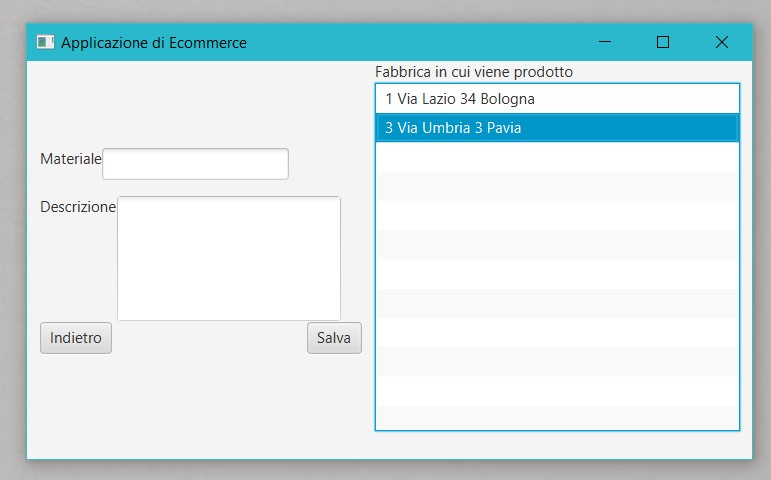
\includegraphics[width=\textwidth]{img/Application/Producer3.jpg}
	\caption{Creazione di una nuovo prodotto}
\end{figure}
\subsection*{Schermate amministratore}
L'amministratore del sistema non è una figura presente negli schemi logici, ma è la persona che si occupa di creare corrieri, clienti e produttori, fabbriche, veicoli e gestioni fabbriche. 
Così facendo queste operazioni possibili nel database vengono rappresentate nell'applicazione. L'unica operazione eseguibile dall'applicazione è l'eliminazione delle entità, 
che essendo un'operazione complessa, vista la necessità di eliminare "a cascata" tutte le entità precedentemente legate al target da eliminare, 
si è deciso di lasciarla per una successiva implementazione, rendendola attualmente possibile solo via query diretta al database. 
Le pagine di creazione e modifica delle entità permettono di inserire i dati relativi alle entità, mantenendo intatti i vincoli espressi nella creazione del database. 
\begin{figure}[H]
	\centering{}
	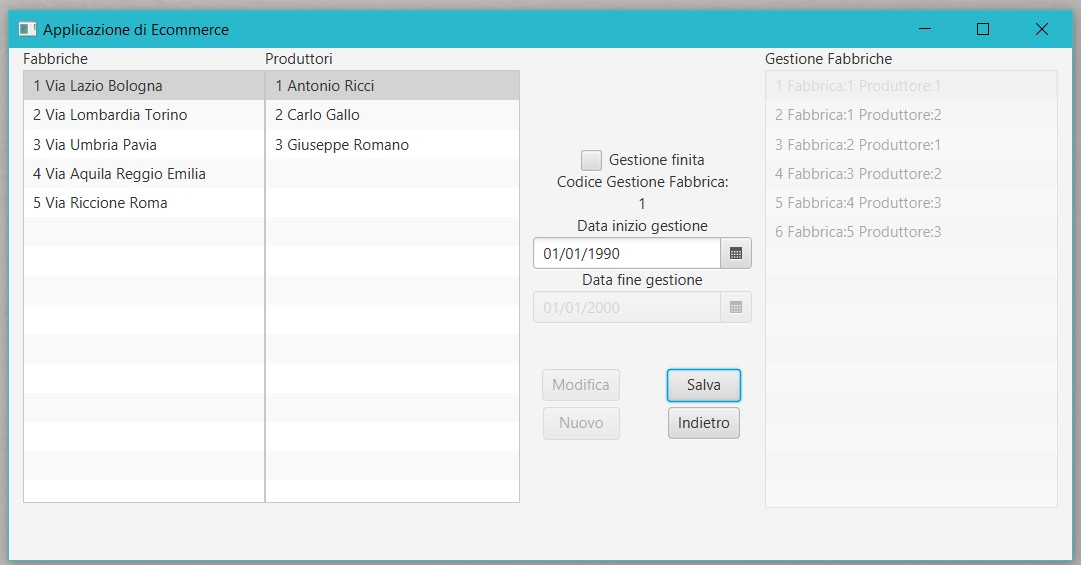
\includegraphics[width=\textwidth]{img/Application/Admin.jpg}
	\caption{Pagina della modifica delle gestioni delle fabbriche}
\end{figure}
In particolare nella gestione delle fabbriche viene implementato il vincolo inespresso che impedisce ad una fabbrica di essere gestita da più produttori in contemporanea 
perchè il salvataggio dei dati avviene solo se i dati sono legali, altrimenti compare un messaggio di errore.
\end{document}